%%%%%%%%%%%%%%%%%%%%%%%%%%%%%%%%%%%%%%%%%%%%%%%%%%%%%%%%%%%%%%%%%%%%%%%%%%%%%%%%%%%%%%%%%%%%%%%%%%%
%%%%%%%%%%%%%%%%%%%%%%%%%%%%%%%%%%%%%%%%%%%%%%%%%%%%%%%%%%%%%%%%%%%%%%%%%%%%%%%%%%%%%%%%%%%%%%%%%%%
%%%%%%%%%%%%%%%%%%%%%%%%%%%%%%%%%%%%%%%%%%%%%%%%%%%%%%%%%%%%%%%%%%%%%%%%%%%%%%%%%%%%%%%%%%%%%%%%%%%
%%%%%%%%%%%%%%%%%%%%%%%%%%%%%%%%%%%%%%%%%%%%%%%%%%%%%%%%%%%%%%%%%%%%%%%%%%%%%%%%%%%%%%%%%%%%%%%%%%%

\chapter{Tablas}

En este ap\'endice se incluyen las gr\'aficas y tablas obtenidas durante el trabajo; todos ellos 
son referidos en la secci\'on de Resultados, pero son presentados como ap\'endice a fin de resaltar 
en el texto las conclusiones obtenidas.

En las primeras tres tablas (\ref{total_gpos_mor}, \ref{total_gpos_nmor}, \ref{total_gpos_total}) 
se muestra el n\'umero total de \'epocas clasificadas como PE para cada sujeto y cada canal para 
las diferentes etapas de sue\~no. En las siguientes tablas (\ref{gpos_mor}, \ref{gpos_nmor}, 
\ref{gpos_total}) se exhibe la misma informaci\'on pero como proporciones, a modo de 
normalizaci\'on entre los diferentes sujetos. Se muestran promedios y desviaciones est\'andar por 
cada grupo.

Posteriormente, en la tabla \ref{comparacion_mor_vs_total} se muestran los resultados de comparar 
la proporci\'on de \'epocas PE durante MOR y NMOR; este an\'alisis se hizo individualmente por cada
sujeto usando la prueba $\chi^{2}$ para proporciones.

%%%%%%%%%%%%%%%%%%%%%%%%%%%%%%%%%%%%%%%%%%%%%%%%%%%%%%%%%%%%%%%%%%%%%%%%%%%%%%%%%%%%%%%%%%%%%%%%%%%

\begin{SidewaysTable}
\centering
\begin{tabular}{c}
\textbf{\'epocas clasificadas como PE, sue\~no MOR}
\vspace{1em}
\end{tabular}
\begin{tabular}{lrrrrrcrrrrcrrr}
\toprule
& \multicolumn{5}{c}{\textbf{Gpo. Control}} && 
  \multicolumn{4}{c}{\textbf{Gpo. PDC}} && 
  \multicolumn{3}{c}{\textbf{Excluidos}}\\
\cmidrule{2-6} \cmidrule{8-11} \cmidrule{13-15}
& \textbf{VCR} & \textbf{MJH} & \textbf{JAE} & \textbf{GHA} & \textbf{MFGR} & \phantom{l}
& \textbf{CLO} & \textbf{RLO} & \textbf{RRU} & \textbf{JGZ} & \phantom{l}
& \textbf{FGH} & \textbf{MGG} & \textbf{EMT} \\
\midrule
\textbf{C3} &6 &18&10&1 &12&&6 &35&16&1 &&2 &28&22 \\
\textbf{C4} &7 &16&4 &2 &10&&4 &40&5 &0 &&1 &23&26 \\
\textbf{CZ} &2 &16&13&2 &8 &&5 &22&4 &1 &&1 &13&19 \\
\rowcolor{gris}
\textbf{F3} &5 &23&10&0 &3 &&7 &43&3 &3 &&6 &14&20 \\
\rowcolor{gris}
\textbf{F4} &11&23&5 &1 &1 &&6 &36&5 &0 &&0 &4 &24 \\
\rowcolor{gris}
\textbf{F7} &5 &15&2 &0 &4 &&1 &18&0 &0 &&0 &2 &24 \\
\rowcolor{gris}
\textbf{F8} &4 &11&6 &1 &3 &&4 &23&1 &0 &&0 &2 &20 \\
\textbf{FP1}&2 &7 &1 &0 &1 &&0 &0 &1 &0 &&22&0 &22 \\
\textbf{FP2}&1 &6 &3 &0 &2 &&1 &15&1 &0 &&0 &1 &18 \\
\textbf{FZ} &11&18&19&0 &6 &&7 &38&2 &2 &&0 &20&23 \\
\rowcolor{gris}
\textbf{O1} &10&20&5 &3 &23&&2 &25&9 &2 &&5 &18&19 \\
\rowcolor{gris}
\textbf{O2} &13&23&3 &3 &21&&3 &34&9 &1 &&1 &12&16 \\
\textbf{P3} &6 &17&2 &2 &26&&5 &33&8 &0 &&1 &24&17 \\
\textbf{P4} &4 &19&4 &5 &18&&4 &27&5 &1 &&4 &15&21 \\
\textbf{PZ} &4 &15&5 &3 &22&&4 &32&4 &0 &&1 &8 &20 \\
\rowcolor{gris}
\textbf{T3} &10&29&1 &8 &26&&10&34&4 &0 &&2 &29&31 \\
\rowcolor{gris}
\textbf{T4} &12&20&2 &3 &21&&3 &35&6 &1 &&0 &10&17 \\
\rowcolor{gris}
\textbf{T5} &10&26&0 &3 &27&&5 &34&5 &2 &&2 &31&19 \\
\rowcolor{gris}
\textbf{T6} &15&18&3 &15&20&&3 &24&4 &2 &&0 &9 &19 \\
\textbf{LOG}&6 &20&8 &0 &9 &&5 &11&2 &0 &&1 &8 &30 \\
\textbf{ROG}&6 &21&17&2 &11&&9 &7 &4 &1 &&0 &19&33 \\
\textbf{EMG}&14&11&0 &0 &17&&14&16&4 &0 &&0&3&7 \\
\rowcolor{gris2}
\textbf{Total}&73&127&171&55&95&&132&99&38&33&&22&166&47 \\
\bottomrule
\end{tabular}
\caption{Total de \'epocas clasificadas como PE en sue\~no MOR, desglosado por canal. En la 
\'ultima fila se reporta el total de \'epocas de sue\~no MOR.
}
\label{total_gpos_mor}
\end{SidewaysTable}

%%%%%%%%%%%%%%%%%%%%%%%%%%%%%%%%%%%%%%%%%%%%%%%%%%%%%%%%%%%%%%%%%%%%%%%%%%%%%%%%%%%%%%%%%%%%%%%%%%%

\begin{SidewaysTable}
\centering
\begin{tabular}{c}
\textbf{\'epocas clasificadas como PE, sue\~no NMOR}
\vspace{1em}
\end{tabular}
\begin{tabular}{lrrrrrcrrrrcrrr}
\toprule
& \multicolumn{5}{c}{\textbf{Gpo. Control}} && 
  \multicolumn{4}{c}{\textbf{Gpo. PDC}} && 
  \multicolumn{3}{c}{\textbf{Excluidos}}\\
\cmidrule{2-6} \cmidrule{8-11} \cmidrule{13-15}
& \textbf{VCR} & \textbf{MJH} & \textbf{JAE} & \textbf{GHA} & \textbf{MFGR} & \phantom{l}
& \textbf{CLO} & \textbf{RLO} & \textbf{RRU} & \textbf{JGZ} & \phantom{l}
& \textbf{FGH} & \textbf{MGG} & \textbf{EMT} \\
\midrule
\textbf{C3} &187&135&100&175&112&&55 &153&76 &56 &&16 &201&478 \\
\textbf{C4} &168&129&89 &156&87 &&36 &135&94 &47 &&7  &207&598 \\
\textbf{CZ} &167&131&88 &107&77 &&54 &145&69 &62 &&8  &180&518 \\
\rowcolor{gris}
\textbf{F3} &168&134&83 &150&73 &&57 &175&79 &68 &&107&143&331 \\
\rowcolor{gris}
\textbf{F4} &180&132&55 &146&24 &&41 &135&80 &49 &&0  &137&549 \\
\rowcolor{gris}
\textbf{F7} &158&137&77 &213&87 &&45 &112&68 &58 &&0  &152&262 \\
\rowcolor{gris}
\textbf{F8} &157&123&30 &168&36 &&41 &96 &86 &48 &&0  &128&574 \\
\textbf{FP1}&163&75 &23 &128&65 &&34 &0  &71 &44 &&381&169&518 \\
\textbf{FP2}&156&82 &44 &116&21 &&33 &99 &26 &44 &&0  &146&449 \\
\textbf{FZ} &170&134&78 &156&51 &&55 &163&91 &65 &&0  &177&533 \\
\rowcolor{gris}
\textbf{O1} &202&174&51 &295&175&&48 &150&92 &96 &&20 &140&675 \\
\rowcolor{gris}
\textbf{O2} &166&165&63 &247&173&&32 &136&70 &106&&22 &161&573 \\
\textbf{P3} &175&122&53 &288&132&&72 &147&108&95 &&29 &212&490 \\
\textbf{P4} &180&136&108&252&140&&56 &135&110&73 &&18 &206&495 \\
\textbf{PZ} &156&131&90 &216&112&&57 &167&112&59 &&15 &177&497 \\
\rowcolor{gris}
\textbf{T3} &181&140&52 &230&171&&81 &112&80 &102&&27 &115&603 \\
\rowcolor{gris}
\textbf{T4} &181&121&35 &182&128&&26 &110&112&87 &&10 &122&531 \\
\rowcolor{gris}
\textbf{T5} &218&146&16 &265&199&&78 &137&104&61 &&19 &208&621 \\
\rowcolor{gris}
\textbf{T6} &218&148&49 &194&181&&38 &118&98 &84 &&18 &209&558 \\
\textbf{LOG}&236&224&214&287&170&&144&185&128&225&&50 &437&820 \\
\textbf{ROG}&236&205&212&334&159&&126&179&110&225&&67 &455&873 \\
\textbf{EMG}&94 &62 &16 &1  &157&&20 &82 &110&10 &&1  &55 &266 \\
\rowcolor{gris2}
\textbf{Total}&788&905&736&1038&727&&812&747&376&1174&&383&864&1376 \\
\bottomrule
\end{tabular}
\caption{Total de \'epocas clasificadas como PE en sue\~no NMOR, desglosado por canal. 
En la \'ultima fila se reporta el total de \'epocas en sue\~no NMOR.
}
\label{total_gpos_nmor}
\end{SidewaysTable}

%%%%%%%%%%%%%%%%%%%%%%%%%%%%%%%%%%%%%%%%%%%%%%%%%%%%%%%%%%%%%%%%%%%%%%%%%%%%%%%%%%%%%%%%%%%%%%%%%%%

\begin{SidewaysTable}
\centering
\begin{tabular}{c}
\textbf{\'epocas clasificadas como PE, todo el registro}
\vspace{1em}
\end{tabular}
\begin{tabular}{lrrrrrcrrrrcrrr}
\toprule
& \multicolumn{5}{c}{\textbf{Gpo. Control}} && 
  \multicolumn{4}{c}{\textbf{Gpo. PDC}} && 
  \multicolumn{3}{c}{\textbf{Excluidos}}\\
\cmidrule{2-6} \cmidrule{8-11} \cmidrule{13-15}
& \textbf{VCR} & \textbf{MJH} & \textbf{JAE} & \textbf{GHA} & \textbf{MFGR} & \phantom{l}
& \textbf{CLO} & \textbf{RLO} & \textbf{RRU} & \textbf{JGZ} & \phantom{l}
& \textbf{FGH} & \textbf{MGG} & \textbf{EMT} \\
\midrule
\textbf{C3} &193&153&110&176&124&&61 &188&92 &57 &&18&229&500 \\
\textbf{C4} &175&145&93 &158&97 &&40 &175&99 &47 &&8&230&624 \\
\textbf{CZ} &169&147&101&109&85 &&59 &167&73 &63 &&9&193&537 \\
\rowcolor{gris}
\textbf{F3} &173&157&93 &150&76 &&64 &218&82 &71 &&113&157&351 \\
\rowcolor{gris}
\textbf{F4} &191&155&60 &147&25 &&47 &171&85 &49 &&0&141&573 \\
\rowcolor{gris}
\textbf{F7} &163&152&79 &213&91 &&46 &130&68 &58 &&0&154&286 \\
\rowcolor{gris}
\textbf{F8} &161&134&36 &169&39 &&45 &119&87 &48 &&0&130&594 \\
\textbf{FP1}&165&82 &24 &128&66 &&34 &0  &72 &44 &&403&169&540 \\
\textbf{FP2}&157&88 &47 &116&23 &&34 &114&27 &44 &&0&147&467 \\
\textbf{FZ} &181&152&97 &156&57 &&62 &201&93 &67 &&0&197&556 \\
\rowcolor{gris}
\textbf{O1} &212&194&56 &298&198&&50 &175&101&98 &&25&158&694 \\
\rowcolor{gris}
\textbf{O2} &179&188&66 &250&194&&35 &170&79 &107&&23&173&589 \\
\textbf{P3} &181&139&55 &290&158&&77 &180&116&95 &&30&236&507 \\
\textbf{P4} &184&155&112&257&158&&60 &162&115&74 &&22&221&516 \\
\textbf{PZ} &160&146&95 &219&134&&61 &199&116&59 &&16&185&517 \\
\rowcolor{gris}
\textbf{T3} &191&169&53 &238&197&&91 &146&84 &102&&29&144&634 \\
\rowcolor{gris}
\textbf{T4} &193&141&37 &185&149&&29 &145&118&88 &&10&132&548 \\
\rowcolor{gris}
\textbf{T5} &228&172&16 &268&226&&83 &171&109&63 &&21&239&640 \\
\rowcolor{gris}
\textbf{T6} &233&166&52 &209&201&&41 &142&102&86 &&18&218&577 \\
\textbf{LOG}&242&244&222&287&179&&149&196&130&225&&51&445&850 \\
\textbf{ROG}&242&226&229&336&170&&135&186&114&226&&67&474&906 \\
\textbf{EMG}&108&73 &16 &1  &174&&34 &98 &114&10 &&1&58&273 \\
\rowcolor{gris2}
\textbf{Total}&861&1032&907&1093&822&&944&846&414&1207&&405&1030&1423 \\
\bottomrule
\end{tabular}
\caption{Total de \'epocas clasificadas como PE en todo el registro, desglosado por canal. 
En la \'ultima fila se reporta el total de \'epocas registradas para cada sujeto.
}
\label{total_gpos_total}
\end{SidewaysTable}

%%%%%%%%%%%%%%%%%%%%%%%%%%%%%%%%%%%%%%%%%%%%%%%%%%%%%%%%%%%%%%%%%%%%%%%%%%%%%%%%%%%%%%%%%%%%%%%%%%%
%%%%%%%%%%%%%%%%%%%%%%%%%%%%%%%%%%%%%%%%%%%%%%%%%%%%%%%%%%%%%%%%%%%%%%%%%%%%%%%%%%%%%%%%%%%%%%%%%%%

\begin{SidewaysTable}
\centering
\begin{tabular}{c}
\textbf{Porcentaje de \'epocas PE, sue\~no MOR}
\vspace{1em}
\end{tabular}
{\footnotesize
\bordes{1.3}
\begin{tabular}{lccccccclcccccclccc}
\toprule
& \multicolumn{7}{c}{\textbf{Gpo. Control}} &&
  \multicolumn{6}{c}{\textbf{Gpo. PDC}} &&
  \multicolumn{3}{c}{\textbf{Excluidos}} \\
\cmidrule{2-8} \cmidrule{10-15} \cmidrule{17-19}
& \textbf{VCR} & \textbf{MJH} & \textbf{JAE} & \textbf{GHA} & \textbf{MFGR} 
    &$\widehat{\mu}$ & $\widehat{\sigma}$ & \phantom{l}
& \textbf{CLO} & \textbf{RLO} & \textbf{RRU} & \textbf{JGZ} 
    &$\widehat{\mu}$ & $\widehat{\sigma}$ & \phantom{l}
& \textbf{FGH} & \textbf{MGG} & \textbf{EMT} \\ 
\midrule
\textbf{C3} &0.082&0.142&0.058&0.018&0.126&0.085&0.050&&0.045&0.354&0.421&0.030&0.213&0.204&&0.091&0.169&0.468 \\
\textbf{C4} &0.096&0.126&0.023&0.036&0.105&0.077&0.045&&0.030&0.404&0.132&0.000&0.141&0.184&&0.045&0.139&0.553 \\
\textbf{CZ} &0.027&0.126&0.076&0.036&0.084&0.070&0.040&&0.038&0.222&0.105&0.030&0.099&0.089&&0.045&0.078&0.404 \\
\rowcolor{gris}
\textbf{F3} &0.068&0.181&0.058&0.000&0.032&0.068&0.069&&0.053&0.434&0.079&0.091&0.164&0.181&&0.273&0.084&0.426 \\
\rowcolor{gris}
\textbf{F4} &0.151&0.181&0.029&0.018&0.011&0.078&0.081&&0.045&0.364&0.132&0.000&0.135&0.162&&0.000&0.024&0.511 \\
\rowcolor{gris}
\textbf{F7} &0.068&0.118&0.012&0.000&0.042&0.048&0.047&&0.008&0.182&0.000&0.000&0.047&0.090&&0.000&0.012&0.511 \\
\rowcolor{gris}
\textbf{F8} &0.055&0.087&0.035&0.018&0.032&0.045&0.027&&0.030&0.232&0.026&0.000&0.072&0.108&&0.000&0.012&0.426 \\
\textbf{FP1}&0.027&0.055&0.006&0.000&0.011&0.020&0.022&&0.000&0.000&0.026&0.000&0.007&0.013&&1.000&0.000&0.468 \\
\textbf{FP2}&0.014&0.047&0.018&0.000&0.021&0.020&0.017&&0.008&0.152&0.026&0.000&0.046&0.071&&0.000&0.006&0.383 \\
\textbf{FZ} &0.151&0.142&0.111&0.000&0.063&0.093&0.062&&0.053&0.384&0.053&0.061&0.138&0.164&&0.000&0.120&0.489 \\
\rowcolor{gris}
\textbf{O1} &0.137&0.157&0.029&0.055&0.242&0.124&0.085&&0.015&0.253&0.237&0.061&0.141&0.121&&0.227&0.108&0.404 \\
\rowcolor{gris}
\textbf{O2} &0.178&0.181&0.018&0.055&0.221&0.130&0.089&&0.023&0.343&0.237&0.030&0.158&0.158&&0.045&0.072&0.340 \\
\textbf{P3} &0.082&0.134&0.012&0.036&0.274&0.108&0.104&&0.038&0.333&0.211&0.000&0.145&0.155&&0.045&0.145&0.362 \\
\textbf{P4} &0.055&0.150&0.023&0.091&0.189&0.102&0.068&&0.030&0.273&0.132&0.030&0.116&0.115&&0.182&0.090&0.447 \\
\textbf{PZ} &0.055&0.118&0.029&0.055&0.232&0.098&0.082&&0.030&0.323&0.105&0.000&0.115&0.146&&0.045&0.048&0.426 \\
\rowcolor{gris}
\textbf{T3} &0.137&0.228&0.006&0.145&0.274&0.158&0.103&&0.076&0.343&0.105&0.000&0.131&0.148&&0.091&0.175&0.660 \\
\rowcolor{gris}
\textbf{T4} &0.164&0.157&0.012&0.055&0.221&0.122&0.086&&0.023&0.354&0.158&0.030&0.141&0.155&&0.000&0.060&0.362 \\
\rowcolor{gris}
\textbf{T5} &0.137&0.205&0.000&0.055&0.284&0.136&0.114&&0.038&0.343&0.132&0.061&0.143&0.139&&0.091&0.187&0.404 \\
\rowcolor{gris}
\textbf{T6} &0.205&0.142&0.018&0.273&0.211&0.170&0.097&&0.023&0.242&0.105&0.061&0.108&0.096&&0.000&0.054&0.404 \\
\textbf{LOG}&0.082&0.157&0.047&0.000&0.095&0.076&0.058&&0.038&0.111&0.053&0.000&0.050&0.046&&0.045&0.048&0.638 \\
\textbf{ROG}&0.082&0.165&0.099&0.036&0.116&0.100&0.047&&0.068&0.071&0.105&0.030&0.069&0.031&&0.000&0.114&0.702 \\
\textbf{EMG}&0.192&0.087&0.000&0.000&0.179&0.091&0.093&&0.106&0.162&0.105&0.000&0.093&0.068&&0.000&0.018&0.149 \\
\bottomrule
\end{tabular}
}
\caption{Proporci\'on estimada de \'epocas PE respecto al total de \'epocas MOR (fase R),
desglosados por canal. Se incluyen medias y desviaciones est\'andar para los grupos Control 
(izquierda) y PDC (centro).}
\label{gpos_mor}
\end{SidewaysTable}

%%%%%%%%%%%%%%%%%%%%%%%%%%%%%%%%%%%%%%%%%%%%%%%%%%%%%%%%%%%%%%%%%%%%%%%%%%%%%%%%%%%%%%%%%%%%%%%%%%%

\begin{SidewaysTable}
\centering
\begin{tabular}{c}
\textbf{Porcentaje de \'epocas PE, sue\~no NMOR}
\vspace{1em}
\end{tabular}
{\footnotesize
\bordes{1.3}
\begin{tabular}{lccccccclcccccclccc}
\toprule
& \multicolumn{7}{c}{\textbf{Gpo. Control}} &&
  \multicolumn{6}{c}{\textbf{Gpo. PDC}} &&
  \multicolumn{3}{c}{\textbf{Excluidos}} \\
\cmidrule{2-8} \cmidrule{10-15} \cmidrule{17-19}
& \textbf{VCR} & \textbf{MJH} & \textbf{JAE} & \textbf{GHA} & \textbf{MFGR} 
    &$\widehat{\mu}$ & $\widehat{\sigma}$ & \phantom{l}
& \textbf{CLO} & \textbf{RLO} & \textbf{RRU} & \textbf{JGZ} 
    &$\widehat{\mu}$ & $\widehat{\sigma}$ & \phantom{l}
& \textbf{FGH} & \textbf{MGG} & \textbf{EMT} \\ 
\midrule
\textbf{C3} &0.237&0.149&0.136&0.169&0.154&0.169&0.040&&0.068&0.205&0.202&0.048&0.131&0.085&&0.042&0.233&0.347 \\
\textbf{C4} &0.213&0.143&0.121&0.150&0.120&0.149&0.038&&0.044&0.181&0.250&0.040&0.129&0.104&&0.018&0.240&0.435 \\
\textbf{CZ} &0.212&0.145&0.120&0.103&0.106&0.137&0.045&&0.067&0.194&0.184&0.053&0.124&0.075&&0.021&0.208&0.376 \\
\rowcolor{gris}
\textbf{F3} &0.213&0.148&0.113&0.145&0.100&0.144&0.044&&0.070&0.234&0.210&0.058&0.143&0.092&&0.279&0.166&0.241 \\
\rowcolor{gris}
\textbf{F4} &0.228&0.146&0.075&0.141&0.033&0.125&0.075&&0.050&0.181&0.213&0.042&0.121&0.088&&0.000&0.159&0.399 \\
\rowcolor{gris}
\textbf{F7} &0.201&0.151&0.105&0.205&0.120&0.156&0.046&&0.055&0.150&0.181&0.049&0.109&0.066&&0.000&0.176&0.190 \\
\rowcolor{gris}
\textbf{F8} &0.199&0.136&0.041&0.162&0.050&0.117&0.070&&0.050&0.129&0.229&0.041&0.112&0.087&&0.000&0.148&0.417 \\
\textbf{FP1}&0.207&0.083&0.031&0.123&0.089&0.107&0.065&&0.042&0.000&0.189&0.037&0.067&0.083&&0.995&0.196&0.376 \\
\textbf{FP2}&0.198&0.091&0.060&0.112&0.029&0.098&0.064&&0.041&0.133&0.069&0.037&0.070&0.044&&0.000&0.169&0.326 \\
\textbf{FZ} &0.216&0.148&0.106&0.150&0.070&0.138&0.055&&0.068&0.218&0.242&0.055&0.146&0.098&&0.000&0.205&0.387 \\
\rowcolor{gris}
\textbf{O1} &0.256&0.192&0.069&0.284&0.241&0.209&0.085&&0.059&0.201&0.245&0.082&0.147&0.090&&0.052&0.162&0.491 \\
\rowcolor{gris}
\textbf{O2} &0.211&0.182&0.086&0.238&0.238&0.191&0.063&&0.039&0.182&0.186&0.090&0.124&0.072&&0.057&0.186&0.416 \\
\textbf{P3} &0.222&0.135&0.072&0.277&0.182&0.178&0.079&&0.089&0.197&0.287&0.081&0.163&0.098&&0.076&0.245&0.356 \\
\textbf{P4} &0.228&0.150&0.147&0.243&0.193&0.192&0.044&&0.069&0.181&0.293&0.062&0.151&0.109&&0.047&0.238&0.360 \\
\textbf{PZ} &0.198&0.145&0.122&0.208&0.154&0.165&0.036&&0.070&0.224&0.298&0.050&0.160&0.120&&0.039&0.205&0.361 \\
\rowcolor{gris}
\textbf{T3} &0.230&0.155&0.071&0.222&0.235&0.182&0.070&&0.100&0.150&0.213&0.087&0.137&0.057&&0.070&0.133&0.438 \\
\rowcolor{gris}
\textbf{T4} &0.230&0.134&0.048&0.175&0.176&0.152&0.068&&0.032&0.147&0.298&0.074&0.138&0.117&&0.026&0.141&0.386 \\
\rowcolor{gris}
\textbf{T5} &0.277&0.161&0.022&0.255&0.274&0.198&0.109&&0.096&0.183&0.277&0.052&0.152&0.099&&0.050&0.241&0.451 \\
\rowcolor{gris}
\textbf{T6} &0.277&0.164&0.067&0.187&0.249&0.189&0.082&&0.047&0.158&0.261&0.072&0.134&0.097&&0.047&0.242&0.406 \\
\textbf{LOG}&0.299&0.248&0.291&0.276&0.234&0.270&0.028&&0.177&0.248&0.340&0.192&0.239&0.074&&0.131&0.506&0.596 \\
\textbf{ROG}&0.299&0.227&0.288&0.322&0.219&0.271&0.046&&0.155&0.240&0.293&0.192&0.220&0.060&&0.175&0.527&0.634 \\
\textbf{EMG}&0.119&0.069&0.022&0.001&0.216&0.085&0.086&&0.025&0.110&0.293&0.009&0.109&0.130&&0.003&0.064&0.193 \\
\bottomrule
\end{tabular}
}
\caption{Proporci\'on estimada de \'epocas PE respecto al total de \'epocas NMOR (fases W y N), 
desglosado por canal. Se incluyen medias y desviaciones est\'andar para los grupos Control y PDC.}
\label{gpos_nmor}
\end{SidewaysTable}

%%%%%%%%%%%%%%%%%%%%%%%%%%%%%%%%%%%%%%%%%%%%%%%%%%%%%%%%%%%%%%%%%%%%%%%%%%%%%%%%%%%%%%%%%%%%%%%%%%%

\begin{SidewaysTable}
\centering
\begin{tabular}{c}
\textbf{Porcentaje de \'epocas PE, todo el registro}
\vspace{1em}
\end{tabular}
{\footnotesize
\bordes{1.3}
\begin{tabular}{lccccccclcccccclccc}
\toprule
& \multicolumn{7}{c}{\textbf{Gpo. Control}} &&
  \multicolumn{6}{c}{\textbf{Gpo. PDC}} &&
  \multicolumn{3}{c}{\textbf{Excluidos}} \\
\cmidrule{2-8} \cmidrule{10-15} \cmidrule{17-19}
& \textbf{VCR} & \textbf{MJH} & \textbf{JAE} & \textbf{GHA} & \textbf{MFGR} 
    &$\widehat{\mu}$ & $\widehat{\sigma}$ & \phantom{l}
& \textbf{CLO} & \textbf{RLO} & \textbf{RRU} & \textbf{JGZ} 
    &$\widehat{\mu}$ & $\widehat{\sigma}$ & \phantom{l}
& \textbf{FGH} & \textbf{MGG} & \textbf{EMT} \\ 
\midrule
\textbf{C3} &0.224&0.148&0.121&0.161&0.151&0.161&0.038&&0.065&0.222&0.222&0.047&0.139&0.096&&0.044&0.222&0.351 \\
\textbf{C4} &0.203&0.141&0.103&0.145&0.118&0.142&0.038&&0.042&0.207&0.239&0.039&0.132&0.106&&0.020&0.223&0.439 \\
\textbf{CZ} &0.196&0.142&0.111&0.100&0.103&0.131&0.040&&0.063&0.197&0.176&0.052&0.122&0.075&&0.022&0.187&0.377 \\
\rowcolor{gris}
\textbf{F3} &0.201&0.152&0.103&0.137&0.092&0.137&0.043&&0.068&0.258&0.198&0.059&0.146&0.098&&0.279&0.152&0.247 \\
\rowcolor{gris}
\textbf{F4} &0.222&0.150&0.066&0.134&0.030&0.121&0.075&&0.050&0.202&0.205&0.041&0.124&0.092&&0.000&0.137&0.403 \\
\rowcolor{gris}
\textbf{F7} &0.189&0.147&0.087&0.195&0.111&0.146&0.047&&0.049&0.154&0.164&0.048&0.104&0.064&&0.000&0.150&0.201 \\
\rowcolor{gris}
\textbf{F8} &0.187&0.130&0.040&0.155&0.047&0.112&0.065&&0.048&0.141&0.210&0.040&0.110&0.081&&0.000&0.126&0.417 \\
\textbf{FP1}&0.192&0.079&0.026&0.117&0.080&0.099&0.061&&0.036&0.000&0.174&0.036&0.062&0.077&&0.995&0.164&0.379 \\
\textbf{FP2}&0.182&0.085&0.052&0.106&0.028&0.091&0.059&&0.036&0.135&0.065&0.036&0.068&0.046&&0.000&0.143&0.328 \\
\textbf{FZ} &0.210&0.147&0.107&0.143&0.069&0.135&0.052&&0.066&0.238&0.225&0.056&0.146&0.099&&0.000&0.191&0.391 \\
\rowcolor{gris}
\textbf{O1} &0.246&0.188&0.062&0.273&0.241&0.202&0.084&&0.053&0.207&0.244&0.081&0.146&0.093&&0.062&0.153&0.488 \\
\rowcolor{gris}
\textbf{O2} &0.208&0.182&0.073&0.229&0.236&0.186&0.066&&0.037&0.201&0.191&0.089&0.129&0.080&&0.057&0.168&0.414 \\
\textbf{P3} &0.210&0.135&0.061&0.265&0.192&0.173&0.078&&0.082&0.213&0.280&0.079&0.163&0.100&&0.074&0.229&0.356 \\
\textbf{P4} &0.214&0.150&0.123&0.235&0.192&0.183&0.046&&0.064&0.191&0.278&0.061&0.149&0.105&&0.054&0.215&0.363 \\
\textbf{PZ} &0.186&0.141&0.105&0.200&0.163&0.159&0.038&&0.065&0.235&0.280&0.049&0.157&0.118&&0.040&0.180&0.363 \\
\rowcolor{gris}
\textbf{T3} &0.222&0.164&0.058&0.218&0.240&0.180&0.074&&0.096&0.173&0.203&0.085&0.139&0.058&&0.072&0.140&0.446 \\
\rowcolor{gris}
\textbf{T4} &0.224&0.137&0.041&0.169&0.181&0.150&0.069&&0.031&0.171&0.285&0.073&0.140&0.113&&0.025&0.128&0.385 \\
\rowcolor{gris}
\textbf{T5} &0.265&0.167&0.018&0.245&0.275&0.194&0.107&&0.088&0.202&0.263&0.052&0.151&0.098&&0.052&0.232&0.450 \\
\rowcolor{gris}
\textbf{T6} &0.271&0.161&0.057&0.191&0.245&0.185&0.083&&0.043&0.168&0.246&0.071&0.132&0.093&&0.044&0.212&0.405 \\
\textbf{LOG}&0.281&0.236&0.245&0.263&0.218&0.249&0.024&&0.158&0.232&0.314&0.186&0.222&0.068&&0.126&0.432&0.597 \\
\textbf{ROG}&0.281&0.219&0.252&0.307&0.207&0.253&0.042&&0.143&0.220&0.275&0.187&0.206&0.056&&0.165&0.460&0.637 \\
\textbf{EMG}&0.125&0.071&0.018&0.001&0.212&0.085&0.086&&0.036&0.116&0.275&0.008&0.109&0.120&&0.002&0.056&0.192 \\
\bottomrule
\end{tabular}
}
\caption{Proporci\'on estimada de \'epocas PE respecto al total de \'epocas registradas (todas las 
fases), desglosado por canal. Se incluyen medias y desviaciones est\'andar para los grupos 
Control y PDC.}
\label{gpos_total}
\end{SidewaysTable}

%%%%%%%%%%%%%%%%%%%%%%%%%%%%%%%%%%%%%%%%%%%%%%%%%%%%%%%%%%%%%%%%%%%%%%%%%%%%%%%%%%%%%%%%%%%%%%%%%%%
%%%%%%%%%%%%%%%%%%%%%%%%%%%%%%%%%%%%%%%%%%%%%%%%%%%%%%%%%%%%%%%%%%%%%%%%%%%%%%%%%%%%%%%%%%%%%%%%%%%

\begin{SidewaysTable}
\centering
\bordes{1.1}
\begin{tabular}{c}
\textbf{Comparaci\'on individual para proporci\'on de \'epocas PE, MOR vs NMOR}
\vspace{1em}
\end{tabular}
\begin{tabular}{lrrrrrcrrrrcrrr}
\toprule
& \multicolumn{5}{c}{\textbf{Gpo. Control}} && 
  \multicolumn{4}{c}{\textbf{Gpo. PDC}} && 
  \multicolumn{3}{c}{\textbf{Excluidos}}\\
\cmidrule{2-6} \cmidrule{8-11} \cmidrule{13-15}
& \textbf{VCR} & \textbf{MJH} & \textbf{JAE} & \textbf{GHA} & \textbf{MFGR} & \phantom{l}
& \textbf{CLO} & \textbf{RLO} & \textbf{RRU} & \textbf{JGZ} & \phantom{l}
& \textbf{FGH} & \textbf{MGG} & \textbf{EMT} \\
\midrule 
\textbf{C3} &** & &*  &** &  &&   &** &*  & && & &  \\
\textbf{C4} &*  & &***&*  &  &&   &***&   & && &*&  \\
\textbf{CZ} &***& &   &   &  &&   &   &   & && &***&  \\
\rowcolor{gris}
\textbf{F3} &** & &   &** &  &&   &***&   & && &*&** \\
\rowcolor{gris}
\textbf{F4} &   & &   &*  &  &&   &***&   & && &***&  \\
\rowcolor{gris}
\textbf{F7} &*  & &***&***&  &&   &   &*  & && &***&*** \\
\rowcolor{gris}
\textbf{F8} &** & &   &** &  &&   &*  &*  & && &***&  \\
\textbf{FP1}&***& &   &*  &* &&   &   &*  & && &***&  \\
\textbf{FP2}&***& &   &*  &  &&   &   &   & && &***&  \\
\textbf{FZ} &   & &   &***&  &&   &***&*  & && &*&  \\
\rowcolor{gris}
\textbf{O1} &*  & &   &***&  &&   &   &   & &&*& &  \\
\rowcolor{gris}
\textbf{O2} &   & &*  &***&  &&   &***&   & && &***& \\ 
\textbf{P3} &*  & &*  &***&  &&   &** &   & && &*&  \\
\textbf{P4} &***& &***&*  &  &&   &   &   & &&*&***&  \\
\textbf{PZ} &** & &***&*  &  &&   &   &*  & && &***&  \\
\rowcolor{gris}
\textbf{T3} &   & &** &   &  &&   &***&   & && & &** \\
\rowcolor{gris}
\textbf{T4} &   & &   &*  &  &&   &***&   & && &*&  \\
\rowcolor{gris}
\textbf{T5} &*  & &   &***&  &&   &***&   & && & &  \\
\rowcolor{gris}
\textbf{T6} &   & &*  &   &  &&   &   &   & && &***&  \\
\textbf{LOG}&***& &***&***&**&&***&** &***&*&& &***&  \\
\textbf{ROG}&***& &***&***&* &&*  &***&*  &*&& &***&  \\
\textbf{EMG}&   & &   &   &  &&***&   &*  & && & &  \\
\rowcolor{gris2}
\textbf{General}& & & & & &&***& &*& && & & \\
\bottomrule
\end{tabular}
\caption{Diferencias significativas para la comparaci\'on entre proporci\'on de \'epocas PE en
sue\~no MOR y NMOR; los asteriscos representan el p-valor con el cual se rechaza la hip\'otesis 
de igualdad: *=0.05 , **=0.01 , ***=0.005}
\label{comparacion_mor_vs_total}
\end{SidewaysTable}

%%%%%%%%%%%%%%%%%%%%%%%%%%%%%%%%%%%%%%%%%%%%%%%%%%%%%%%%%%%%%%%%%%%%%%%%%%%%%%%%%%%%%%%%%%%%%%%%%%%
%%%%%%%%%%%%%%%%%%%%%%%%%%%%%%%%%%%%%%%%%%%%%%%%%%%%%%%%%%%%%%%%%%%%%%%%%%%%%%%%%%%%%%%%%%%%%%%%%%%

\chapter{Compilados gr\'aficos}

En este ap\'endice se muestran los compilados gr\'aficos mencionados en la parte de resultados,
y que representan la
distribuci\'on temporal y pseudo-espacial de las ocurrencia de \'epocas PSG dentro de los registros 
para cada paciente. 

Primeramente se presentan los compilados gr\'aficos en los que se ha destacado el sue\~no MOR;
posteriormente se presentan los mismos gr\'aficos resaltando los patrones visuales
propuestos, que parecen estar relacionados con la aparici\'on de sue\~no MOR.

\begin{figure}
\centering
\begin{tabular}{ll}
\Large{\textbf{Grupo Control}}
\\
\begin{tabular}{c}
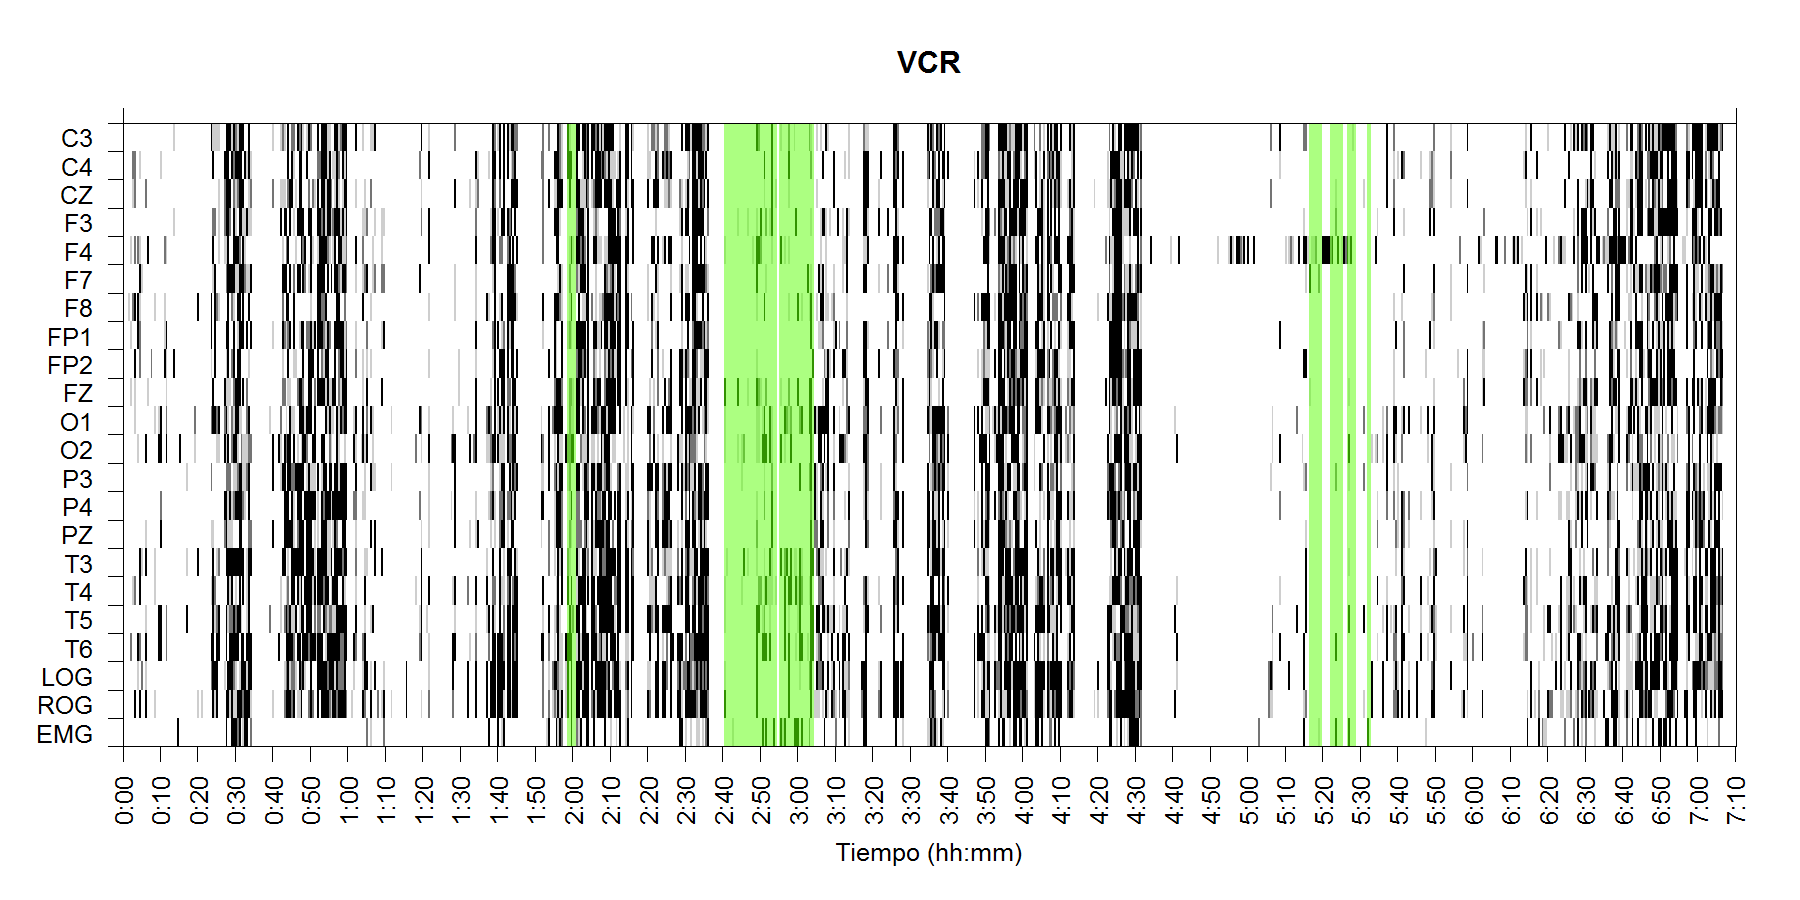
\includegraphics[width=0.8\linewidth]
{./img_ejemplos/VCNNS1_est.png} 
\end{tabular}
\end{tabular}
\label{grf_VCR}
\end{figure}

\begin{figure}
\centering
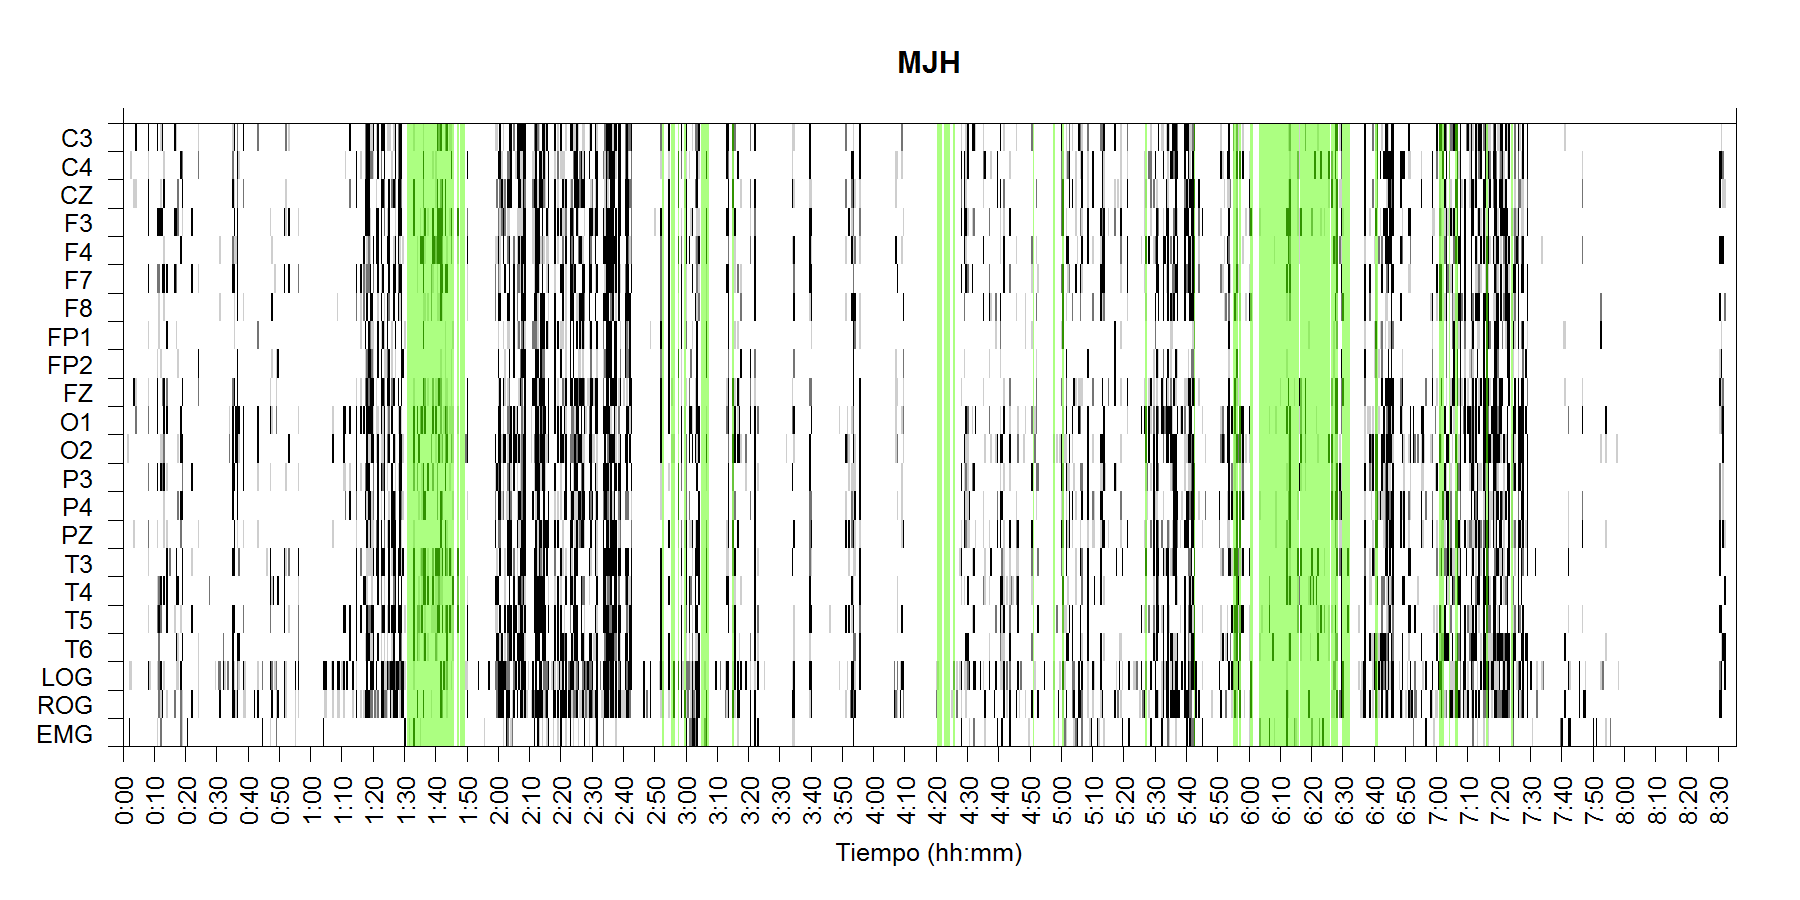
\includegraphics[width=0.8\linewidth]
{./img_ejemplos/MJNNVIGILOS_est.png} 
\label{grf_MJH}
\end{figure}

\begin{figure}
\centering
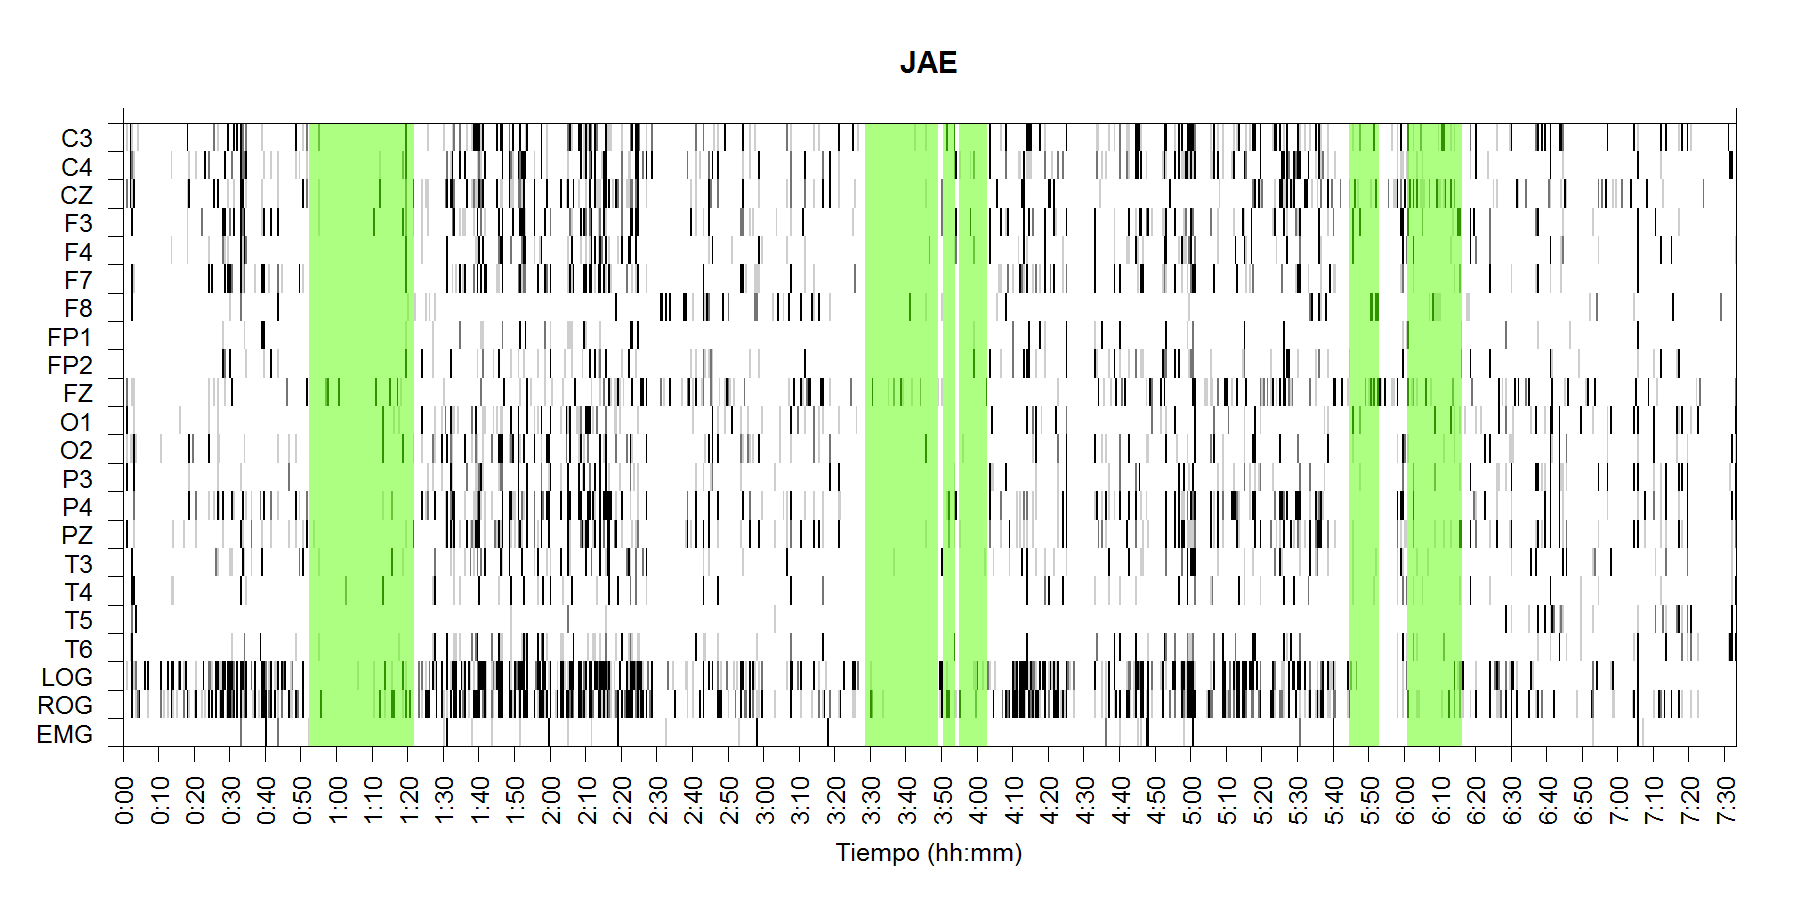
\includegraphics[width=0.8\linewidth]
{./img_ejemplos/JANASUE_est.png} 
\label{grf_JAE}
\end{figure}

\begin{figure}
\centering
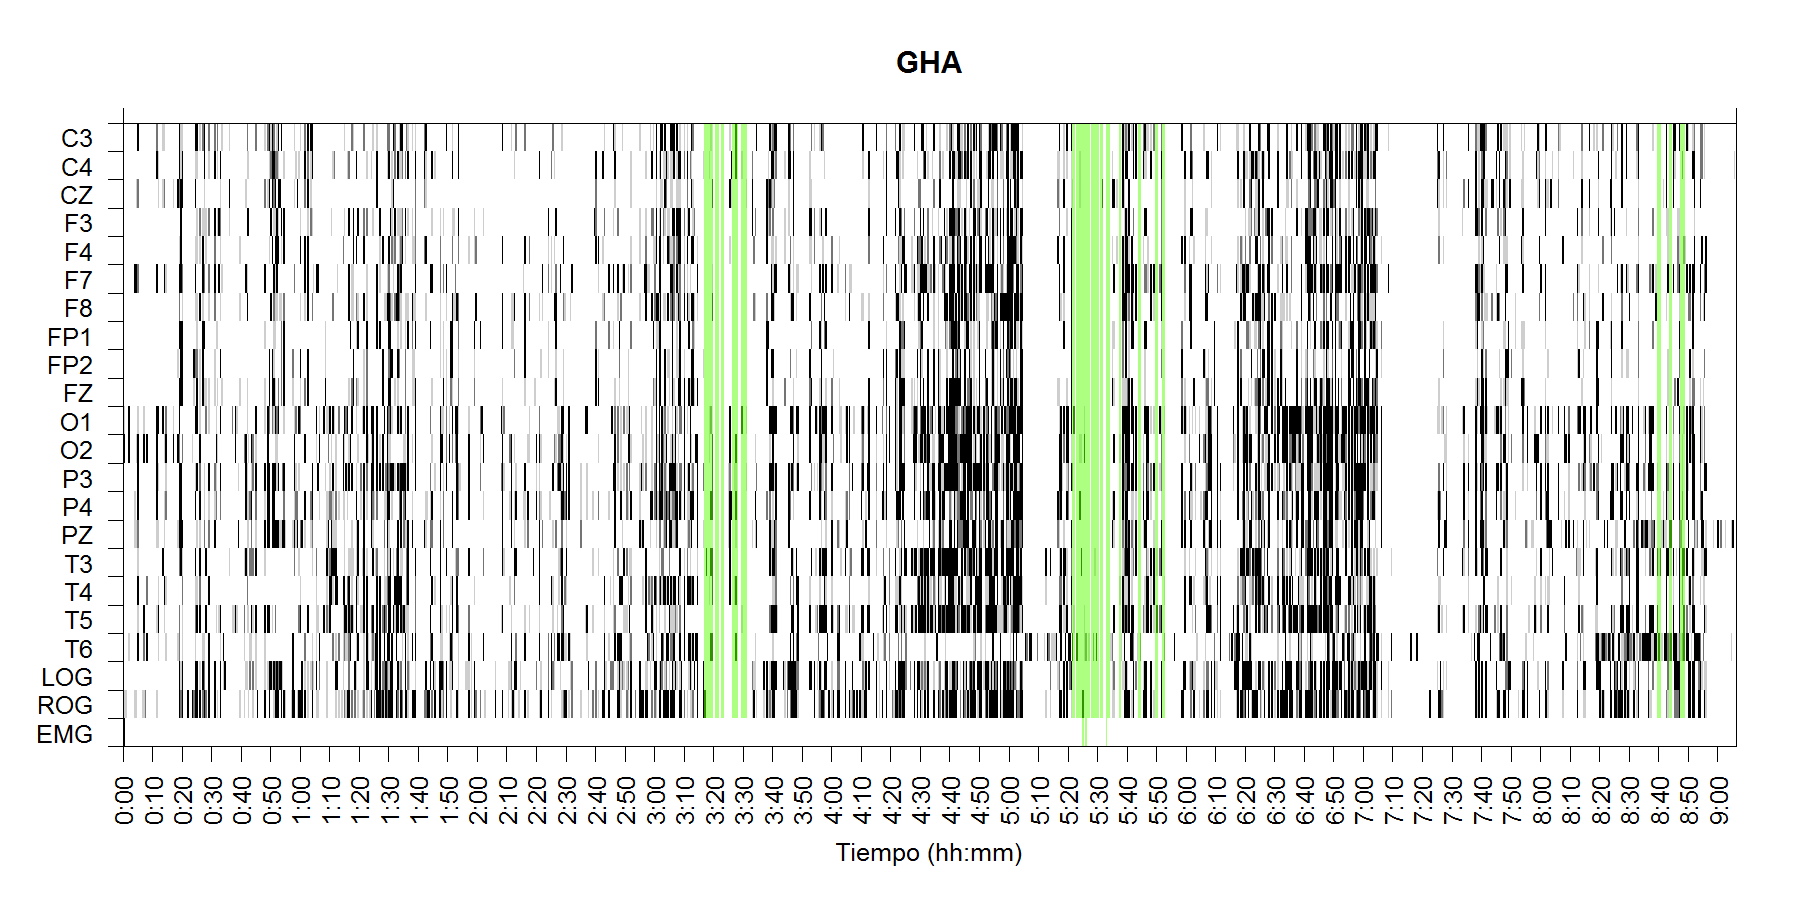
\includegraphics[width=0.8\linewidth]
{./img_ejemplos/GH24031950SUENNO_est.png} 
\label{grf_GHA}
\end{figure}

\begin{figure}
\centering
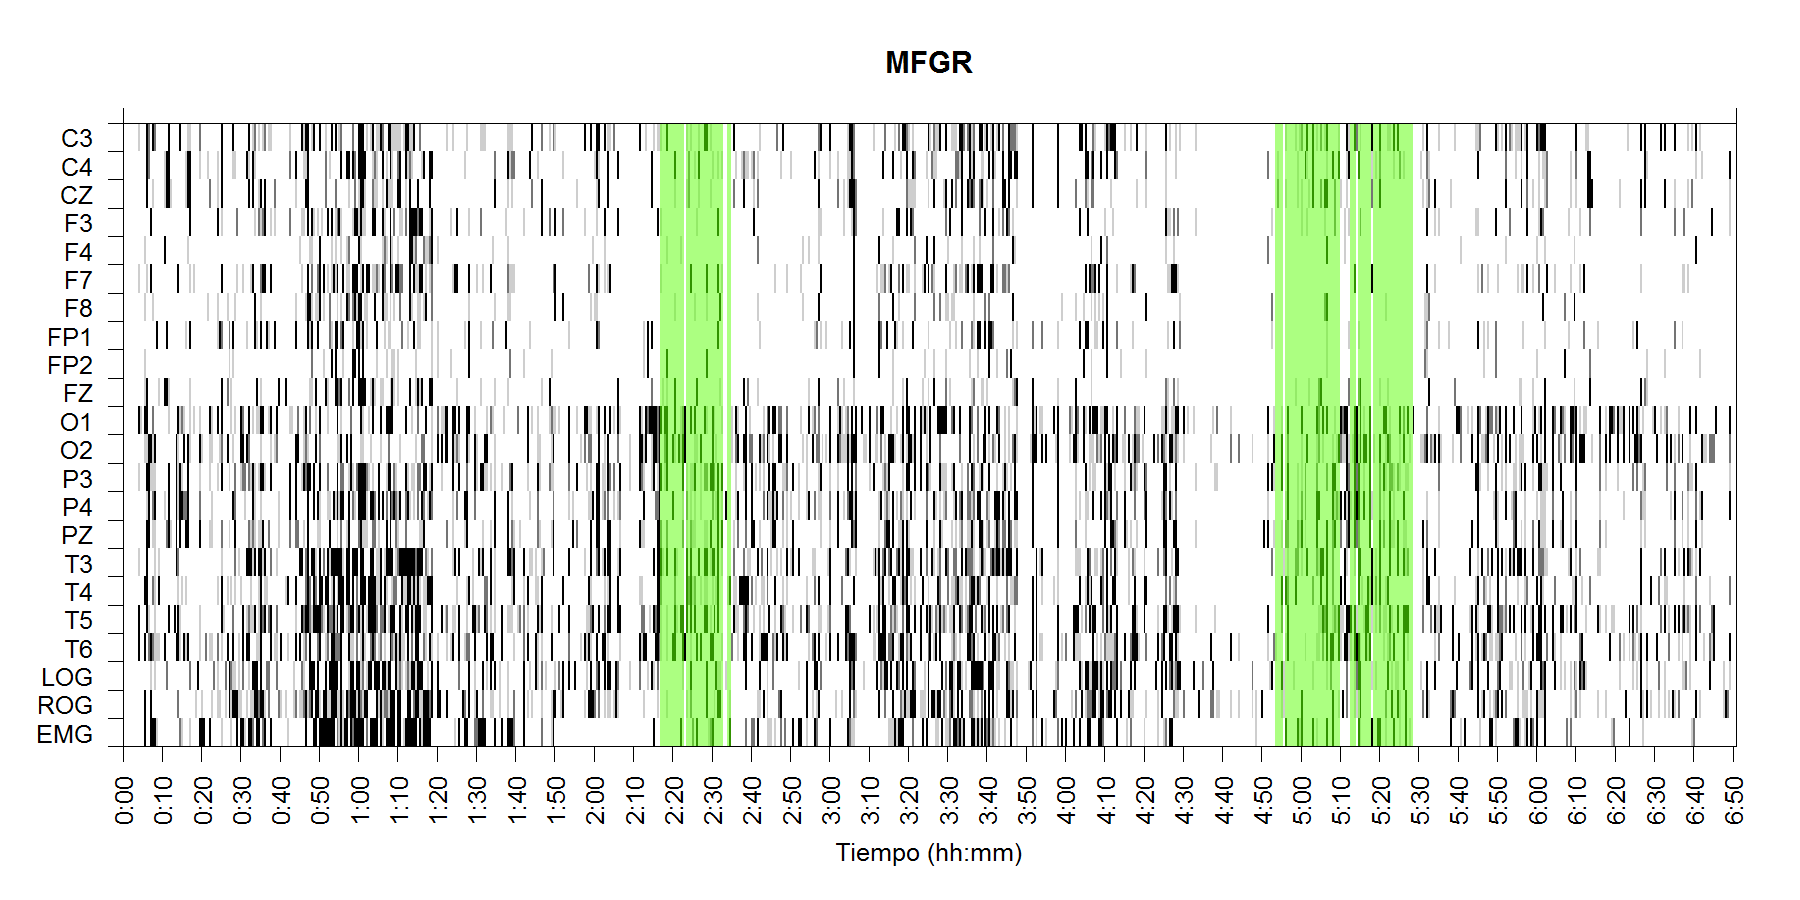
\includegraphics[width=0.8\linewidth]
{./img_ejemplos/GURM251148SUE_est.png} 
\label{grf_MFGR}
\end{figure}

%%%%%%%%%%%%%%%%%%%%%%%%%%%%%%%%%%%%%%%%%%%%%%%%%
%%%%%%%%%%%%%%%%%%%%%%%%%%%%%%%%%%%%%%%%%%%%%%%%%

\begin{figure}
\Large{\textbf{Grupo PDC}}
\end{figure}

\begin{figure}
\centering
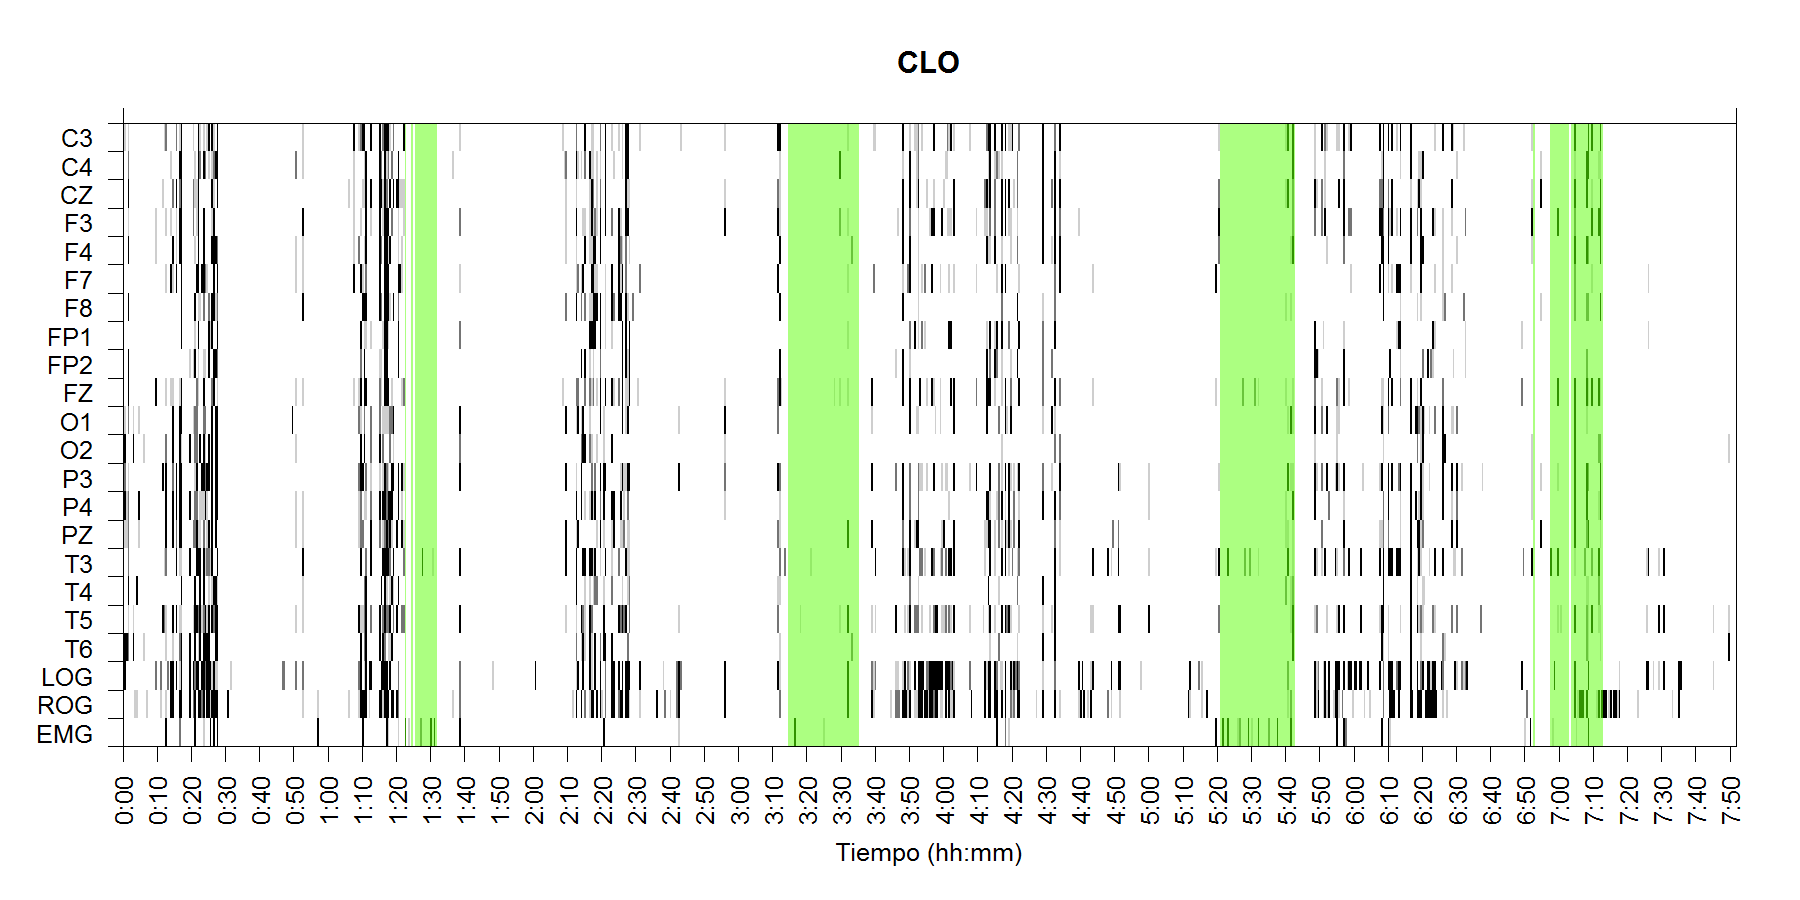
\includegraphics[width=0.8\linewidth]
{./img_ejemplos/CLMN10SUE_est.png} 
\label{grf_CLO}
\end{figure}

\begin{figure}
\centering
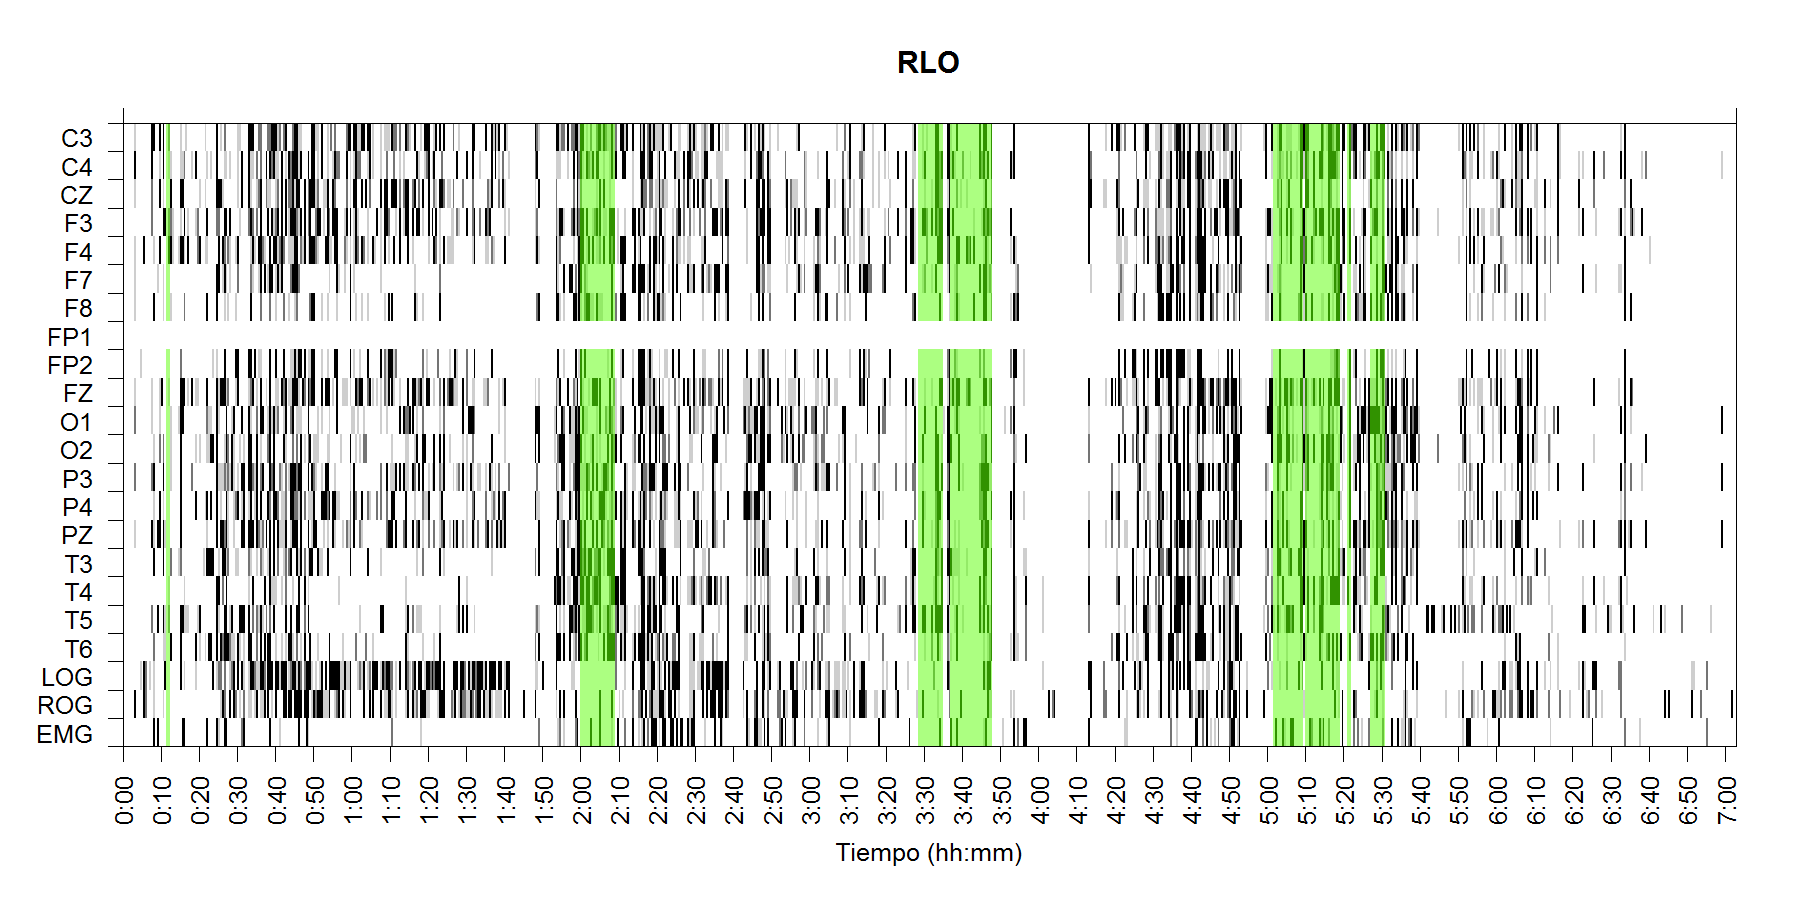
\includegraphics[width=0.8\linewidth]
{./img_ejemplos/RLMN10SUE_est.png} 
\label{grf_RLO}
\end{figure}

\begin{figure}
\centering
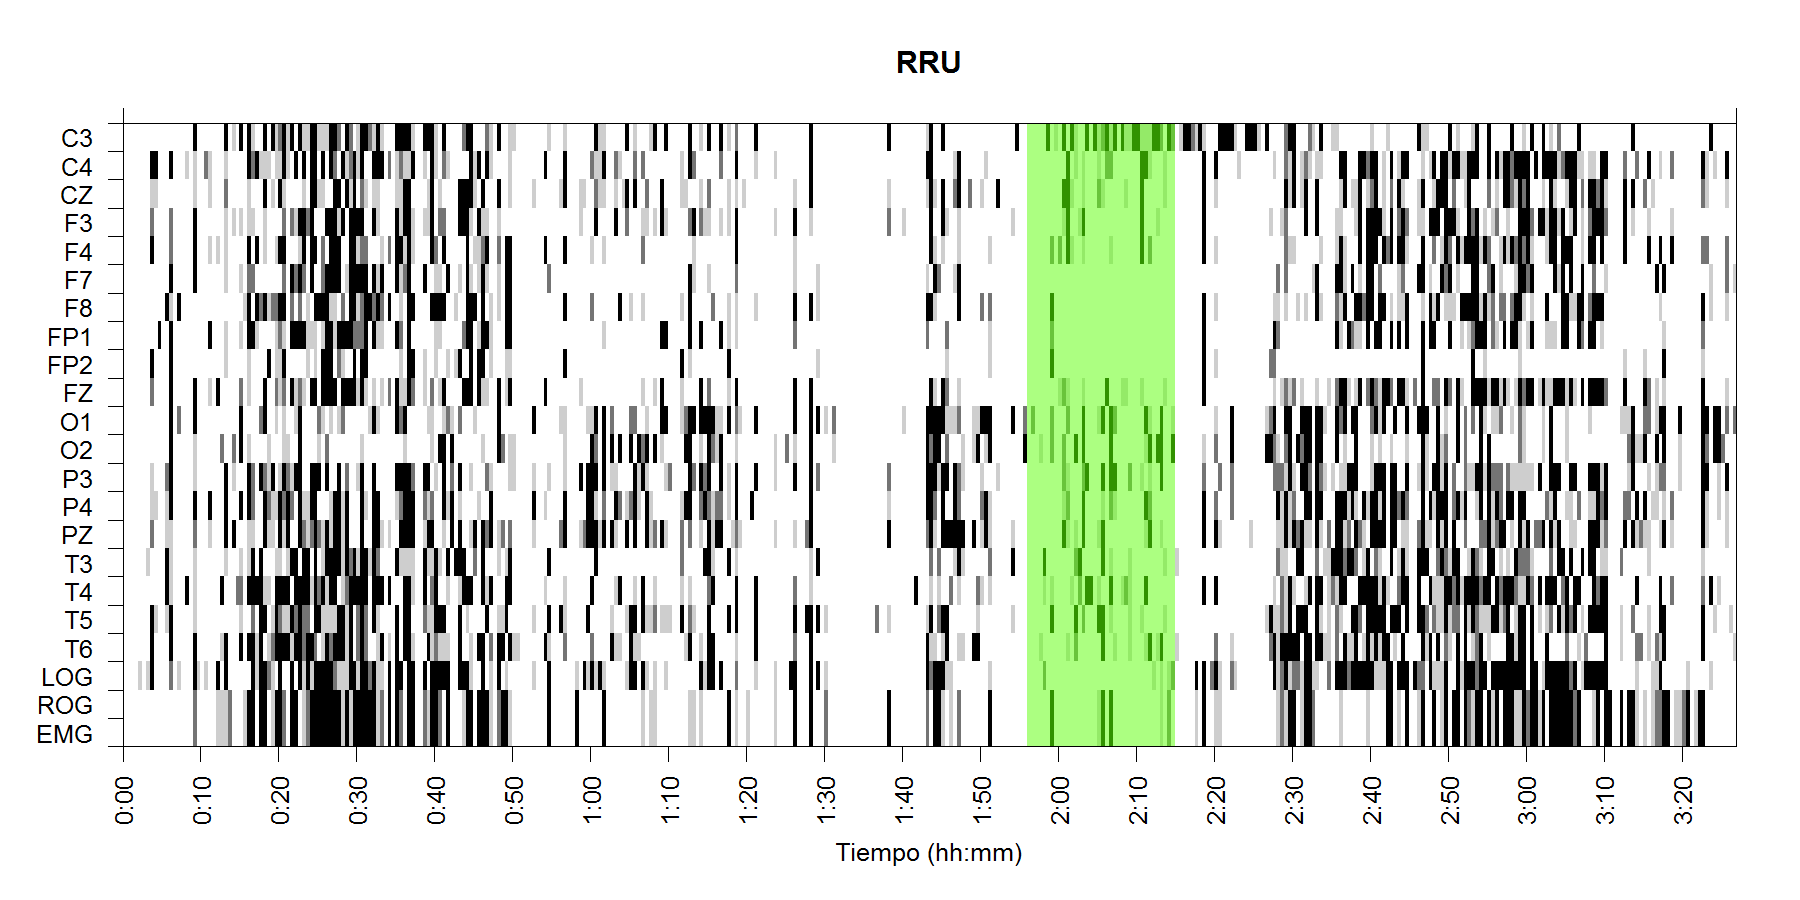
\includegraphics[width=0.8\linewidth]
{./img_ejemplos/RRMNS_est.png} 
\label{grf_RRU}
\end{figure}

\begin{figure}
\centering
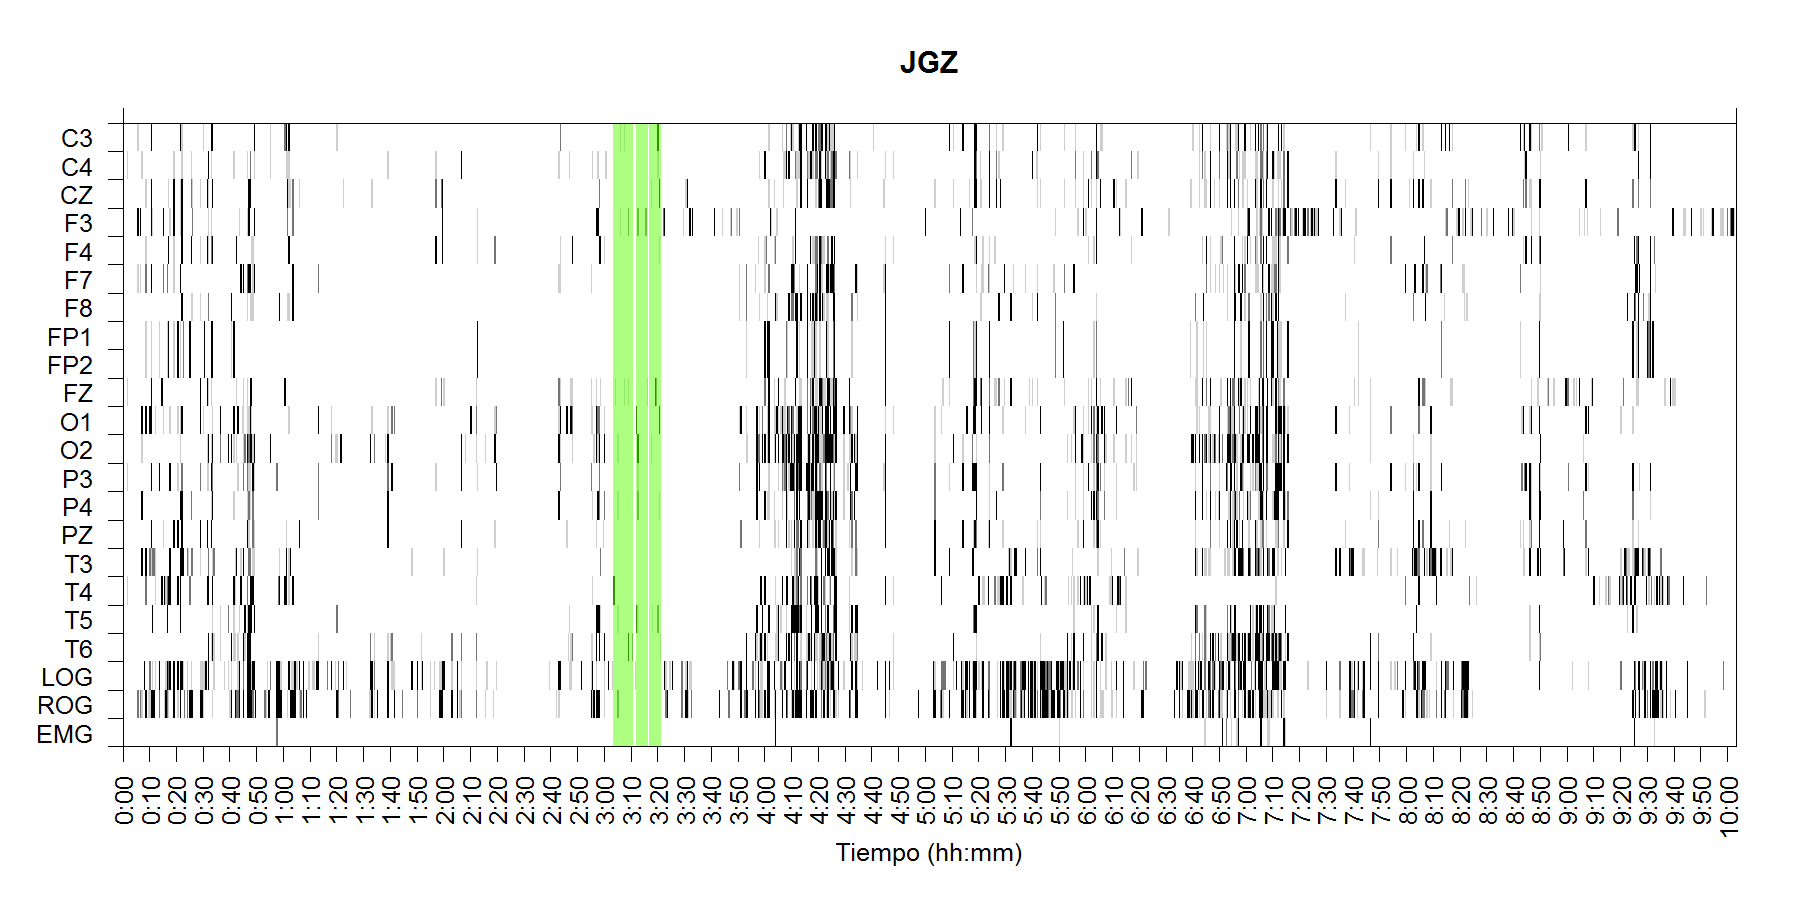
\includegraphics[width=0.8\linewidth]
{./img_ejemplos/JGMN6SUE_est.png} 
\label{grf_JGZ}
\end{figure}

%%%%%%%%%%%%%%%%%%%%%%%%%%%%%%%%%%%%%%%%%%%%%%%%%
%%%%%%%%%%%%%%%%%%%%%%%%%%%%%%%%%%%%%%%%%%%%%%%%%

\begin{figure}
\Large{\textbf{Sujetos excluidos}}
\end{figure}

\begin{figure}
\centering
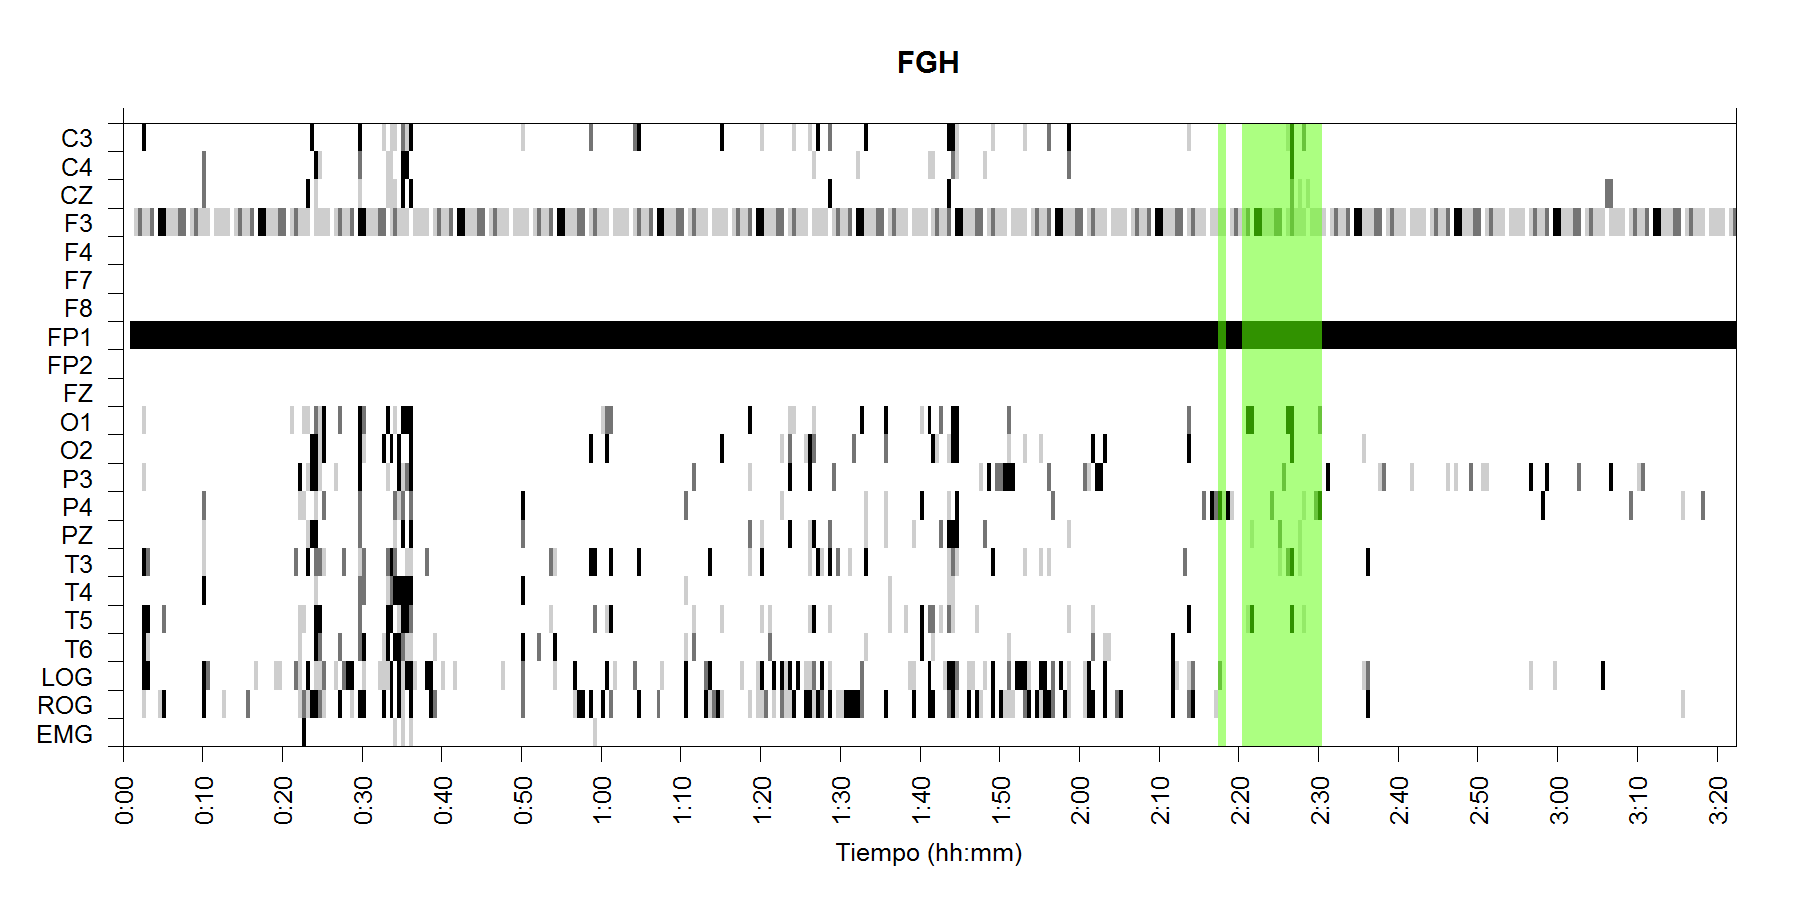
\includegraphics[width=0.8\linewidth]
{./img_ejemplos/FGHSUE_est.png} 
\label{grf_FGH}
\end{figure}

\begin{figure}
\centering
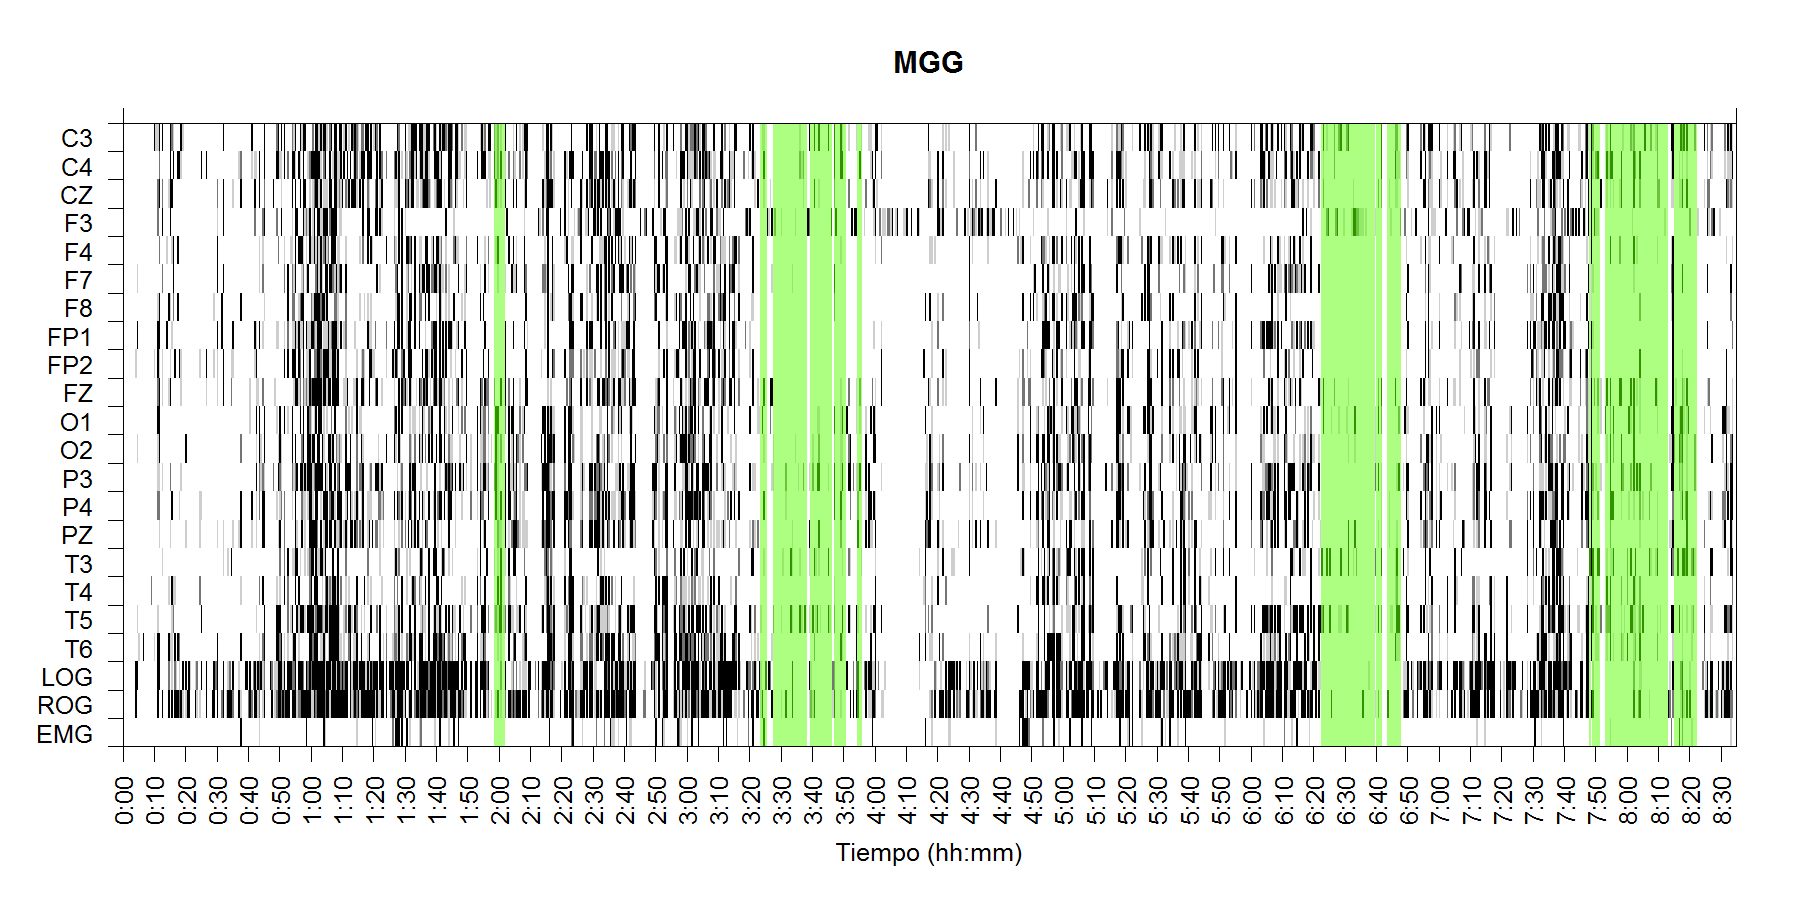
\includegraphics[width=0.8\linewidth]
{./img_ejemplos/MGNA5SUE_est.png} 
\label{grf_MGG}
\end{figure}

\begin{figure}
\centering
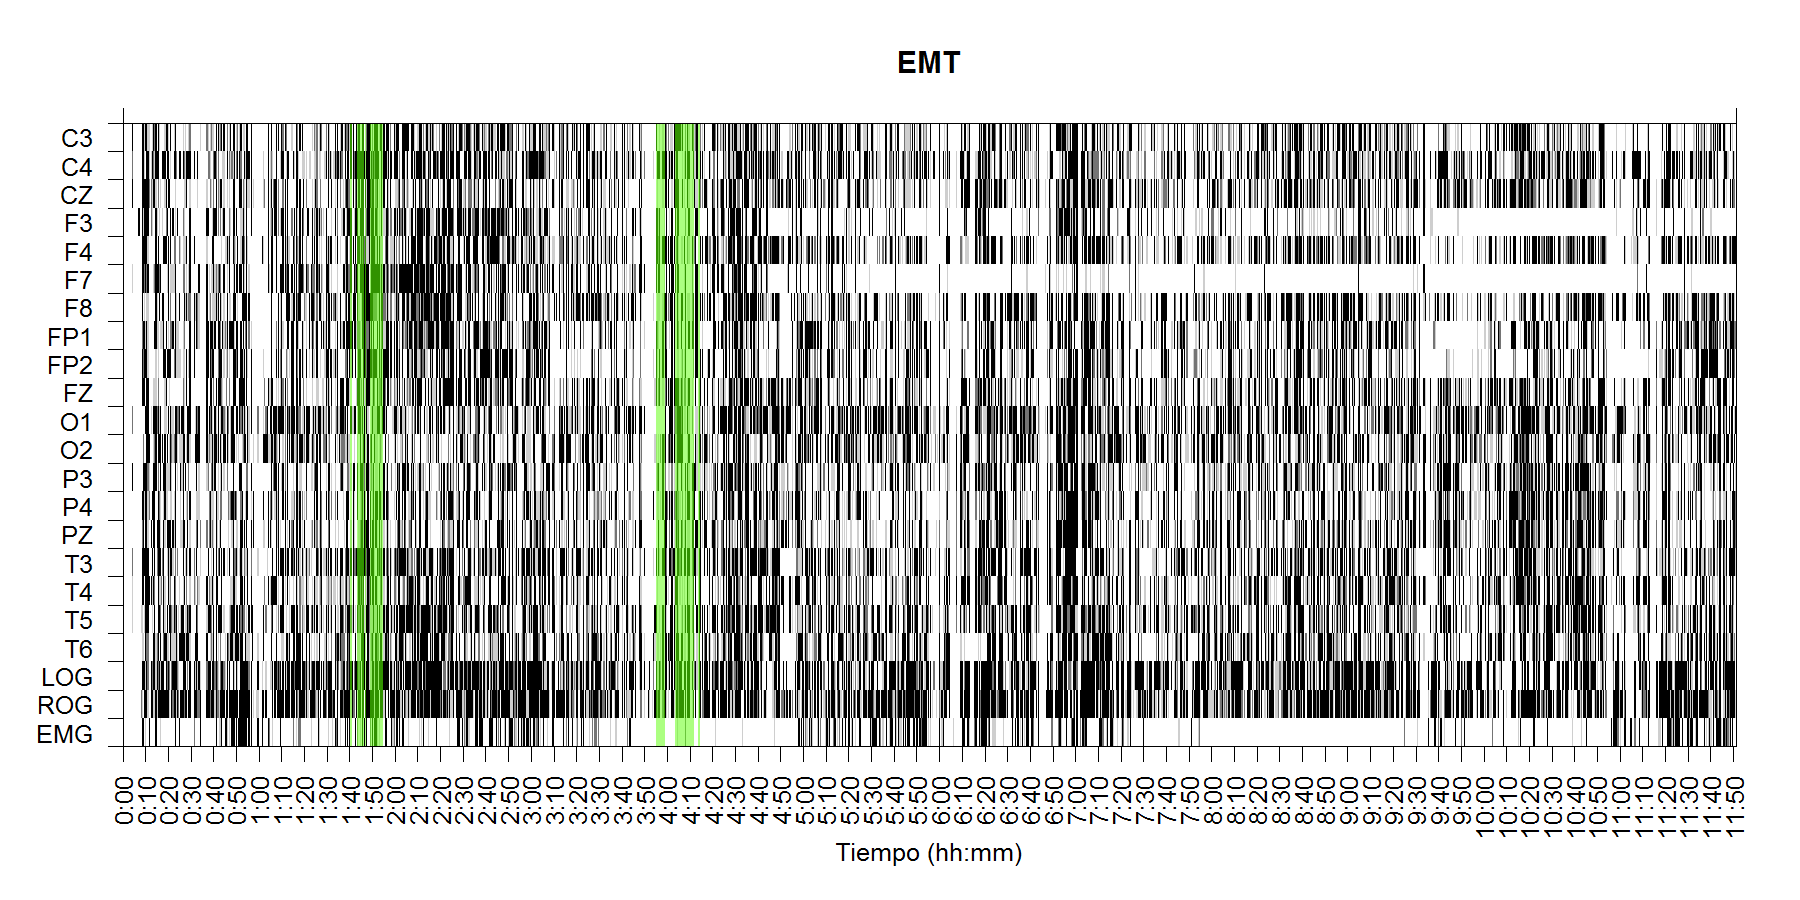
\includegraphics[width=0.8\linewidth]
{./img_ejemplos/EMNNS_est.png} 
\label{grf_EMT}
\end{figure}

%%%%%%%%%%%%%%%%%%%%%%%%%%%%%%%%%%%%%%%%%%%%%%%%%
%%%%%%%%%%%%%%%%%%%%%%%%%%%%%%%%%%%%%%%%%%%%%%%%%

\begin{figure}
\bordes{1.5}
\begin{tabular}{l}
\Large{\textbf{Patrones visuales}}\\
\begin{tabular}{c}
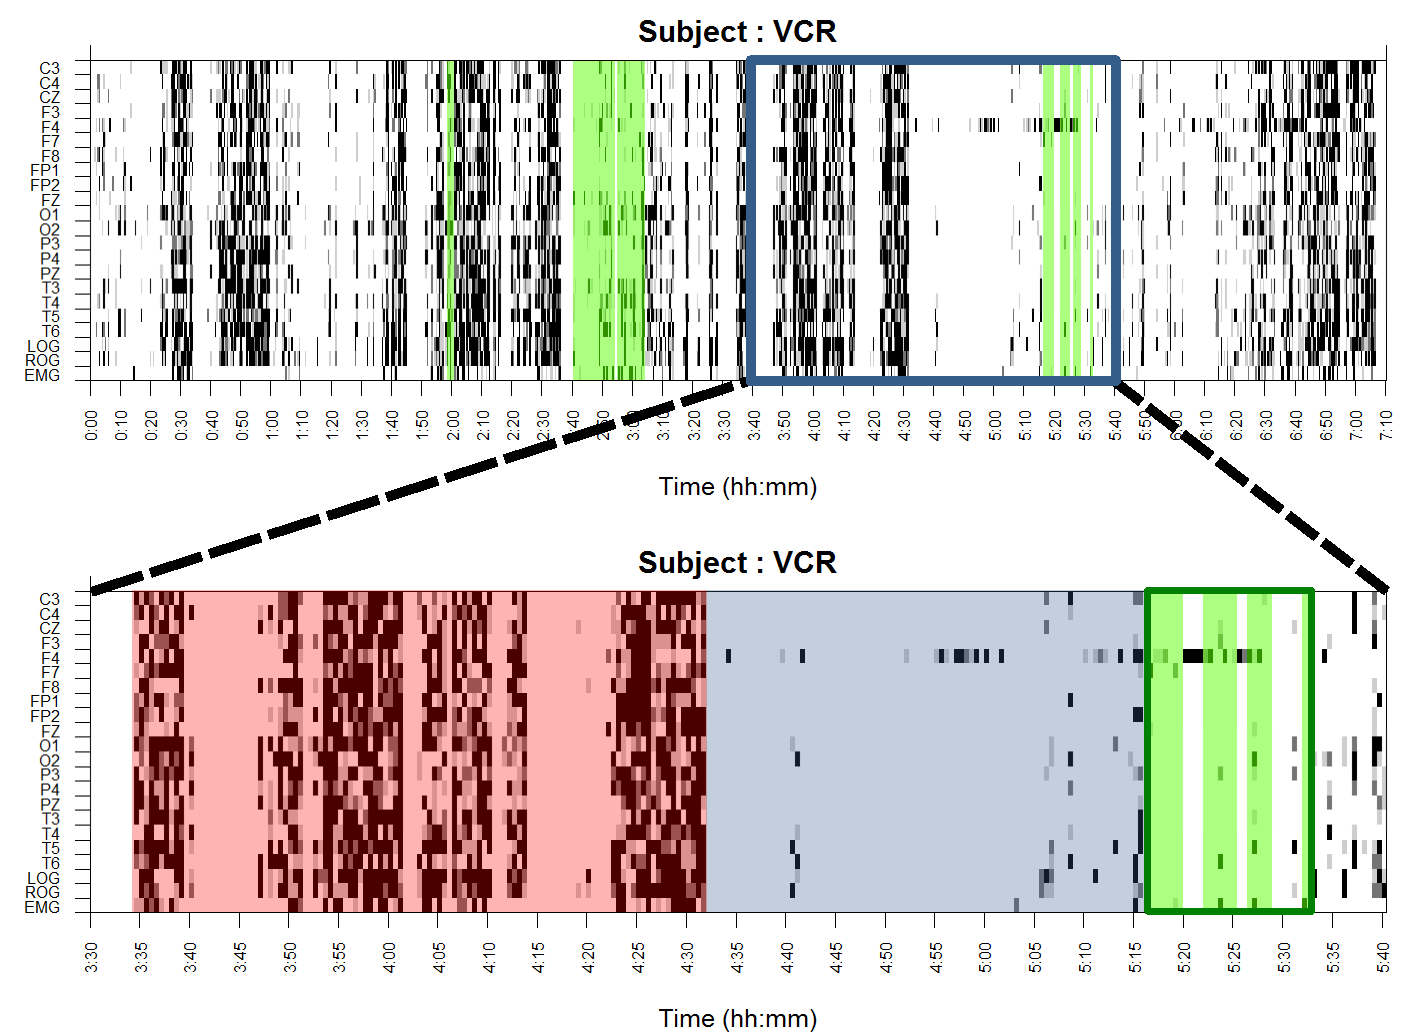
\includegraphics[width=0.45\textwidth]
{./img_ejemplos/zoom_VCR.pdf}
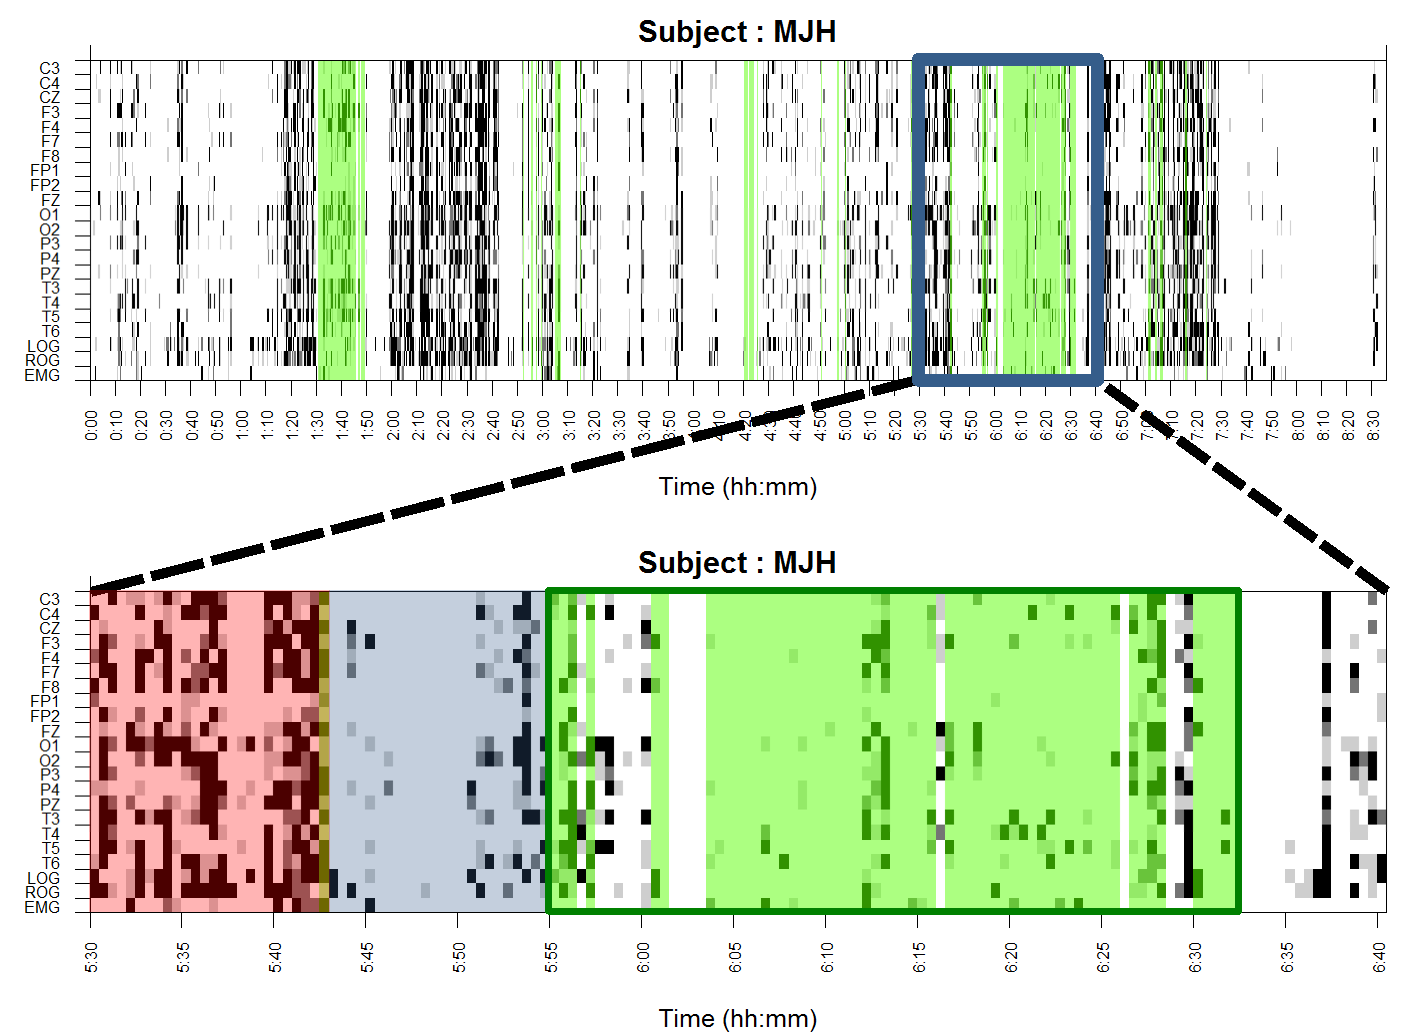
\includegraphics[width=0.45\textwidth]
{./img_ejemplos/zoom_MJH.pdf}
\\
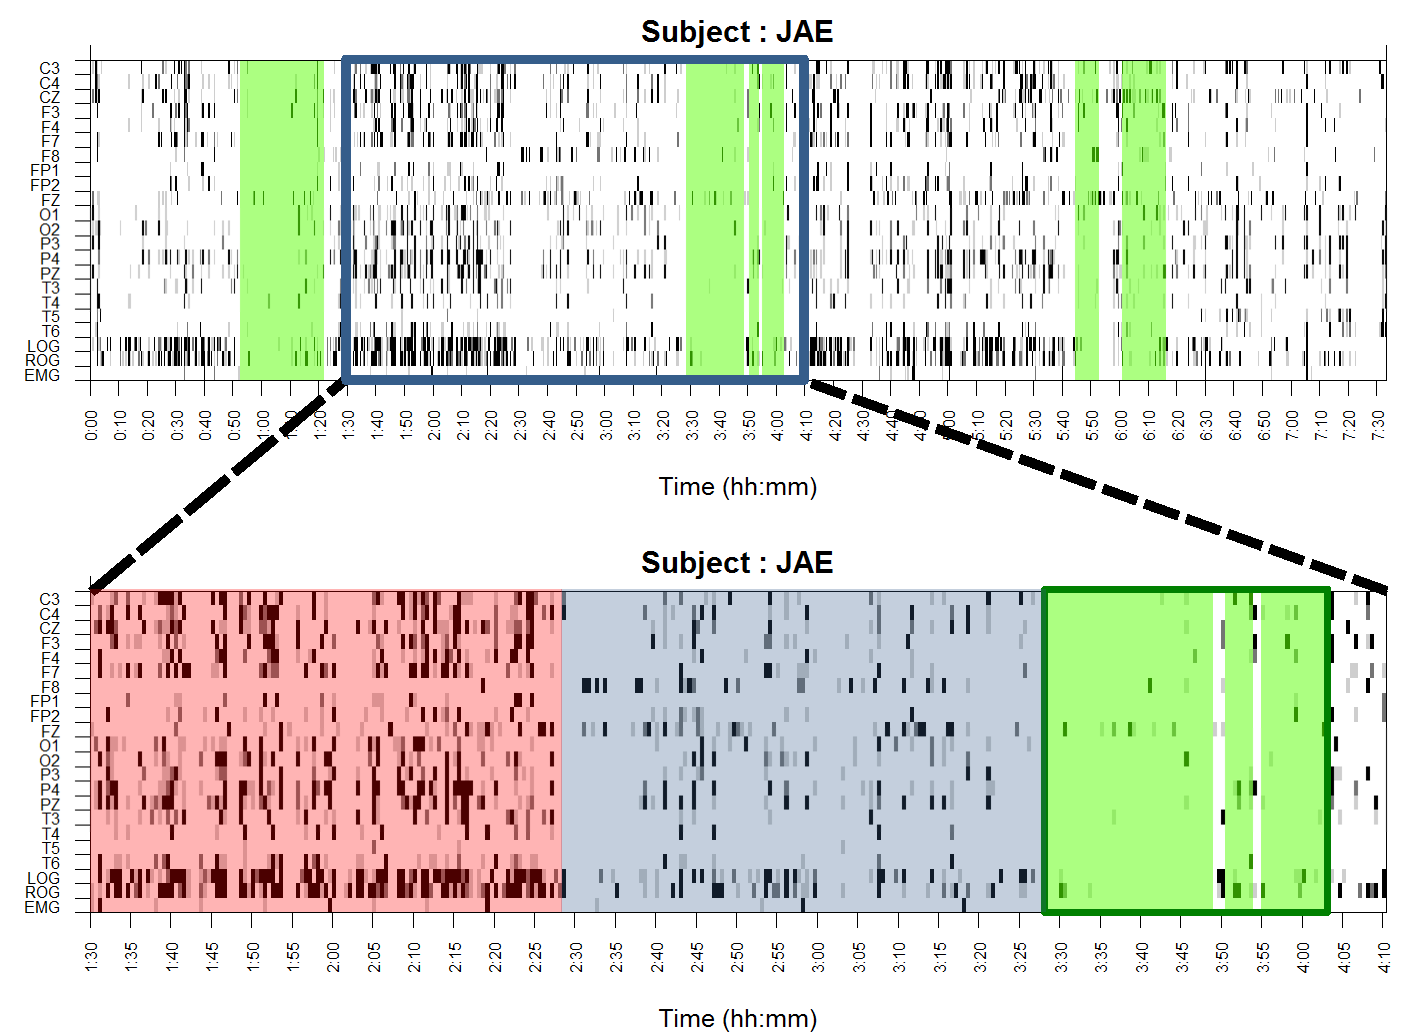
\includegraphics[width=0.45\textwidth]
{./img_ejemplos/zoom_JAE.pdf}
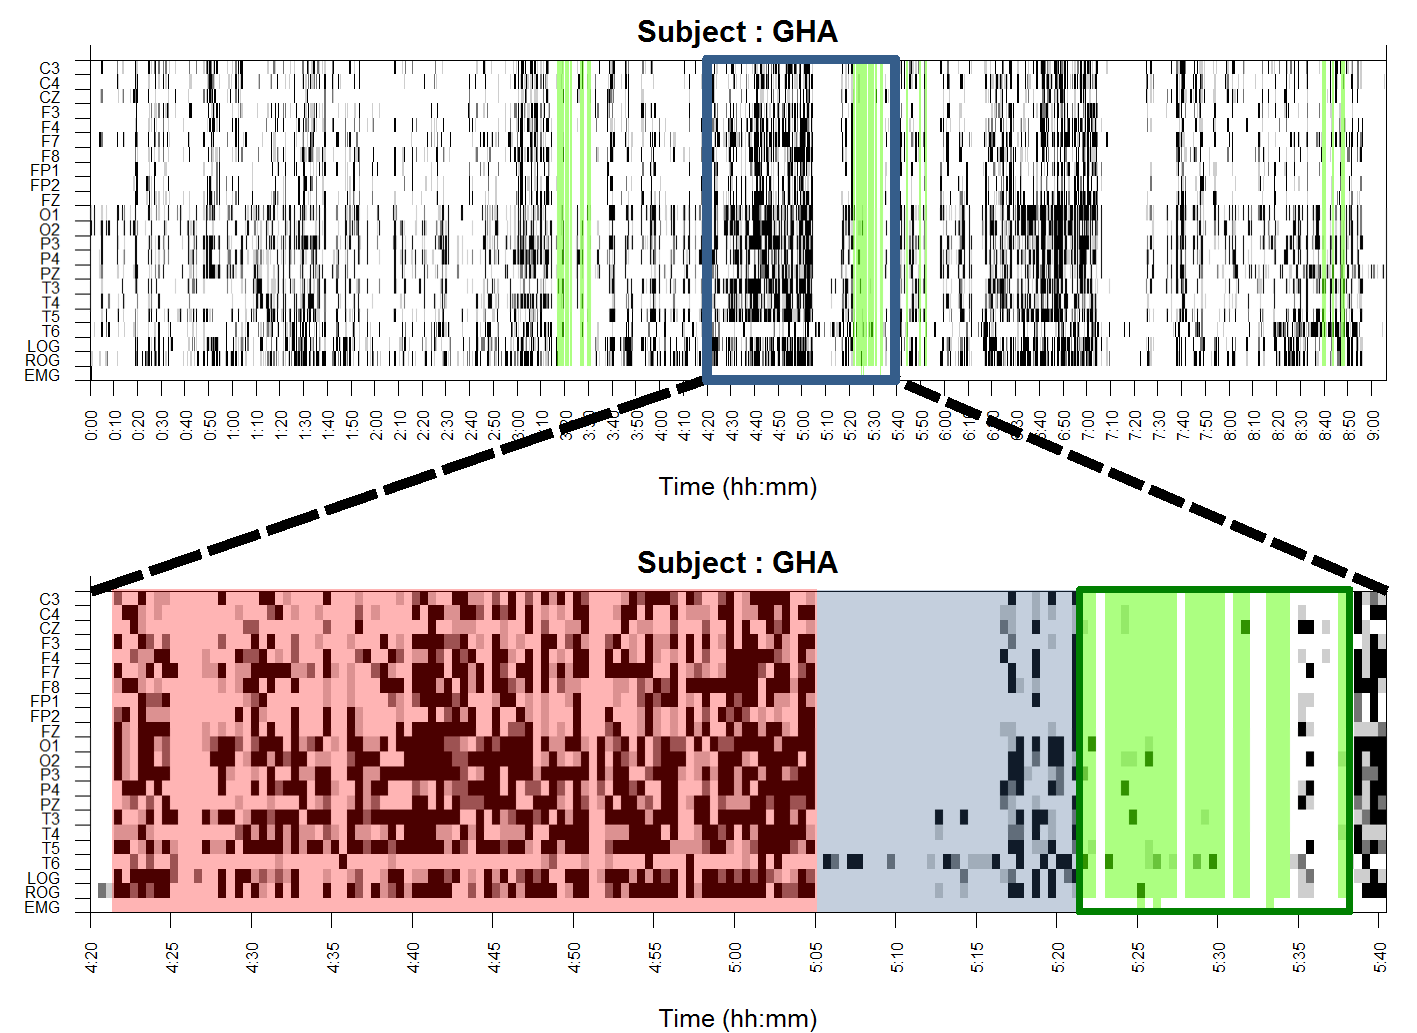
\includegraphics[width=0.45\textwidth]
{./img_ejemplos/zoom_GHA.pdf}
\\
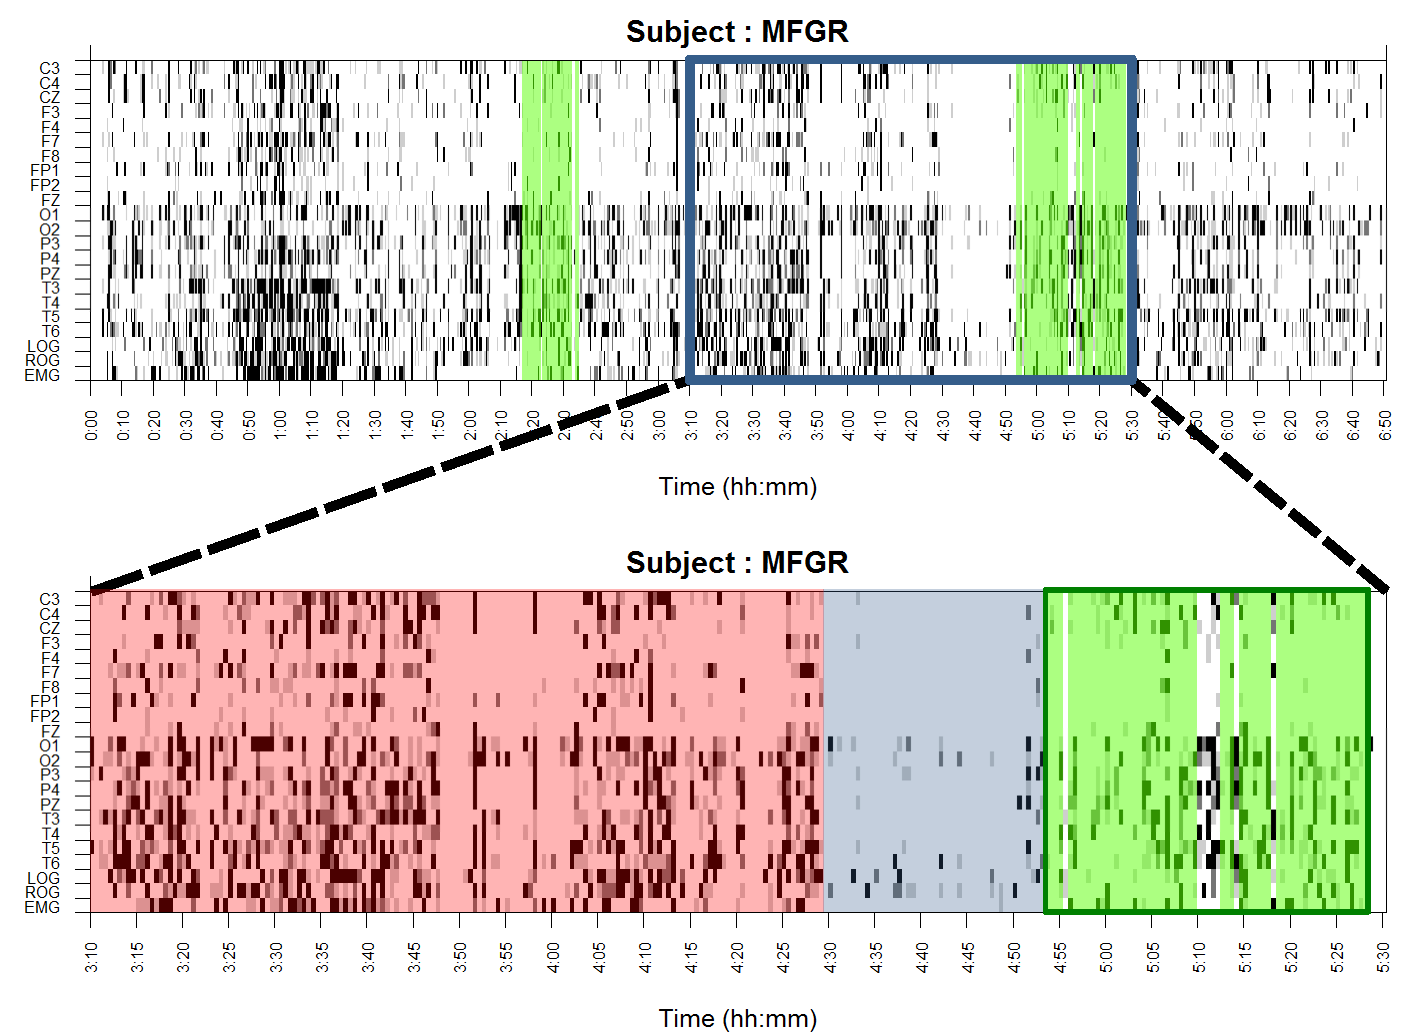
\includegraphics[width=0.45\textwidth]
{./img_ejemplos/zoom_MFGR.pdf}
\end{tabular}
\end{tabular}
\end{figure}

%%%%%%%%%%%%%%%%%%%%%%%%%%%%%%%%%%%%%%%%%%%%%%%%%%%%%%%%%%%%%%%%%%%%%%%%%%%%%%%%%%%%%%%%%%%%%%%%%%%
%%%%%%%%%%%%%%%%%%%%%%%%%%%%%%%%%%%%%%%%%%%%%%%%%%%%%%%%%%%%%%%%%%%%%%%%%%%%%%%%%%%%%%%%%%%%%%%%%%%
%%%%%%%%%%%%%%%%%%%%%%%%%%%%%%%%%%%%%%%%%%%%%%%%%%%%%%%%%%%%%%%%%%%%%%%%%%%%%%%%%%%%%%%%%%%%%%%%%%%
%%%%%%%%%%%%%%%%%%%%%%%%%%%%%%%%%%%%%%%%%%%%%%%%%%%%%%%%%%%%%%%%%%%%%%%%%%%%%%%%%%%%%%%%%%%%%%%%%%%
